\documentclass[11pt]{amsart}
\usepackage[margin=1.15in]{geometry}
\usepackage{amssymb,amsmath,mathtools}
\usepackage{graphicx,booktabs,array}
\usepackage[hidelinks]{hyperref}
\usepackage[expansion=false]{microtype}

\newtheorem{theorem}{Theorem}[section]
\newtheorem{proposition}[theorem]{Proposition}
\newtheorem{lemma}[theorem]{Lemma}
\newtheorem{corollary}[theorem]{Corollary}
\newtheorem{mainthm}{Theorem}
\renewcommand{\themainthm}{\Alph{mainthm}}
\theoremstyle{definition}
\newtheorem{definition}[theorem]{Definition}
\newtheorem{remark}[theorem]{Remark}
\newtheorem{hypothesis}{Hypothesis}
\renewcommand{\thehypothesis}{R}

\newcommand{\ZZ}{\mathbb{Z}}
\newcommand{\QQ}{\mathbb{Q}}
\newcommand{\CC}{\mathbb{C}}
\newcommand{\Phit}{\widetilde\Phi}
\newcommand{\cB}{\mathcal B}
\newcommand{\cH}{\mathcal H}
\newcommand{\fE}{\mathfrak E}
\newcommand{\vt}{\vartheta}
\newcommand{\pA}{\phi_{-2,1}}
\newcommand{\pB}{\phi_{0,1}}
\newcommand{\e}{\mathbf e}
\newcommand{\Dexact}{800}
\newcommand{\Norbits}{22972}
\newcommand{\Qmaxexact}{28}
\newcommand{\zenodoDOI}{10.5281/zenodo.XXXXXXX}

\setlength{\emergencystretch}{2.5em}
\hbadness=2000
\raggedbottom
\begin{document}

\title[Single-centred indices of the $\ZZ_2$ CHL model]{Every Single-Centred Black Hole Index\\ of the $\mathbb Z_2$ CHL Model Is Positive}

\author{Deep Bhattacharjee}
\address{Formerly, Electro-Gravitational Space Propulsion Laboratory (EGSPL), Bhubaneswar, Odisha 751030, India}
\address{Formerly, University of Calcutta (Heramba Chandra College), 23/49 Gariahat Road, Golpark, Kolkata 700029, West Bengal, India}
\email{d.bhattacharjee@erl-forschung.de}
\email{itsdeep@live.com}
\email{egspl@proton.me (GitHub-related contact; GitHub account creelie)}
\urladdr{https://orcid.org/0000-0003-0466-750X}

\begin{abstract}
Every single-centred black hole index of the $\ZZ_2$ CHL model is positive. The proof rests on an exact Rademacher expansion at level two.

\medskip\noindent\textbf{Keywords:} CHL models; single-centred black holes; mock Jacobi forms.

\smallskip\noindent\textbf{MSC 2020:} 11F50 (primary); 11F37, 11F30, 81T30, 83E30.

\smallskip\noindent\textbf{PACS:} 11.25.-w; 04.70.Dy; 11.25.Mj; 02.10.De.
\end{abstract}

\maketitle

\section{Introduction}\label{sec:intro}

A quarter-BPS dyon of $\mathcal N=4$ string theory in four dimensions carries an electric charge $Q$ and a magnetic charge $P$, and the protected index that counts such states is the helicity trace $B_6$. When the charges admit a single-centred black hole whose only hair are the zero modes of the broken supersymmetries, the twelve fermion zero modes fix the sign of the trace, and the horizon degrees of freedom contribute $-B_6>0$. Sen turned this observation into a conjecture about Fourier coefficients of Siegel modular forms \cite{Sen11}: the index $d^*(Q,P)$ of the single-centred black hole, extracted from the inverse of the dyon partition function with the contour of the attractor region, is positive.\footnote{Sen checked the sign on the charges of his Tables~1 to~5, for the heterotic string on $T^6$ and for the CHL models of orders $2,3,5,7$, and stated the conjecture for all charges in the cones (3.7)--(3.12) of \cite{Sen11}. The entropy function and attractor background behind the statement are reviewed in \cite{Sen08}.}

For type~II string theory on $K3\times T^2$, where the partition function is the Igusa cusp form $\Phi_{10}$ \cite{DVV97,SSY06,GN97}, the conjecture is settled. Bringmann and Murthy proved it for the two lowest magnetic charges $P^2=2,4$ by writing the finite parts of the first two Fourier--Jacobi coefficients of $1/\Phi_{10}$ through class numbers \cite{BM13}. Rossell\'o then treated all charges, by writing the single-centred index as a mixed Rademacher series and showing that one of its terms dominates the others; the existence of such series on $SL_2(\ZZ)$ is due to Bringmann and Manschot \cite{BMa13}, and Ferrari and Reys used them for these black holes \cite{FR17}. The CHL models \cite{CHL95} are the $\ZZ_N$ orbifolds of type~IIB on $K3\times T^2$ in which the $\ZZ_N$ acts on $K3$ by a symplectic automorphism and on $T^2$ by a shift; their partition functions $\Phit_k$ are Siegel modular forms of weight $k$ for subgroups of $Sp(2,\ZZ)$ \cite{JS06,DJS06,DS06,DN07}.\footnote{For $N=2$ the model is the heterotic string on $T^6$ obtained from the $E_8\times E_8$ string by exchanging the two $E_8$ factors together with a half shift on a circle \cite{CHL95}; for the ten-dimensional $E_8\times E_8$ theory and its relation to M-theory see \cite{SBBT26}. Background on the involutions of $K3$ surfaces and on Calabi--Yau threefolds fibred by $K3$ surfaces, which underlie the dual type~II description, is in \cite{BN26,Bha22}.} Bhand, Sen and Singh showed that the Fourier--Jacobi coefficients of $1/\Phit_k$ are meromorphic Jacobi forms, split them into an Appell--Lerch polar part and a mock Jacobi finite part, and identified the single-centred index with the Fourier coefficients of the finite part on an explicit set of charges \cite[Theorem~5.4]{BSS25}. Cardoso, Nampuri and Rossell\'o computed the polar coefficients of these finite parts through continued fractions and wrote the immortal index as a Rademacher series, taking the existence of such an expansion at level $N$ as an assumption \cite{CNR21}.

This paper settles the $\ZZ_2$ CHL model. It has $k=6$, duality group $\Gamma_1(2)$, and charges normalised so that $m=Q^2$, $n=P^2/2$ and $\ell=Q\cdot P$ are integers; the discriminant is $D=Q^2P^2-(Q\cdot P)^2=2mn-\ell^2$.

\begin{mainthm}\label{thm:all}
In the $\ZZ_2$ CHL model the single-centred index $d^*(Q,P)$ is positive for every charge with $D>0$.
\end{mainthm}

The proof has two halves. The first is an exact formula for the coefficients of the finite parts.

\begin{mainthm}\label{thm:radB}
For every $m\ge1$ the coefficients $c^F_m(n,\ell)$ of the finite part of the $m$-th Fourier--Jacobi coefficient of $1/\Phit_6$ with $D=2mn-\ell^2>0$ are given by an absolutely convergent vector-valued Rademacher series over the three cosets of $\Gamma^0(2)$ in $SL_2(\ZZ)$, with Bessel terms $I_{15/2}$ from the principal parts and correction terms $I_8$ and $I_{17/2}$ from the shadow. Its principal parts at the cusps $0$ and $\infty$ are explicit sums over Farey walls.
\end{mainthm}

The precise statement is Theorem~\ref{thm:rad}. The wall sums at the cusp $0$ have the shape of the continued-fraction formula of Cardoso, Nampuri and Rossell\'o; we prove them, and their counterpart at the cusp $\infty$, by following the Fourier coefficients of $1/\Phit_6$ across the walls of its poles, which are the Farey geodesics with an even denominator (Figure~\ref{fig:chambers}), and of a second product at the cusp $0$ across all Farey geodesics. The expansion itself comes from the circle method of Rademacher and Zuckerman \cite{RZ38,Zuc39}, applied to the theta coefficients of the finite parts once the Appell--Lerch sum has been completed in the manner of Zwegers \cite{Zwe02}; the completion is proved directly, by a Mordell integral, and the transformation law in all three frames follows from the product formula alone, without any statement about Siegel modular forms.

The second half is the sign. Write $x=\sqrt D/m$ and $\theta=\pi\ell/m$, and let $\mathcal E(D,m)$ be the contribution of the most polar term at the cusp $0$, an explicit multiple of a Bessel function $I_{15/2}$. Every charge has, in its duality orbit or after the Fricke exchange of $Q^2$ and $P^2/2$, a representative with $m\le n$ and $0\le\ell\le m$ (Proposition~\ref{prop:reduction}); then $x\ge1$. The terms of the Rademacher series attached to the leading family of Farey walls, those with the matrix $\begin{psmallmatrix}1&0\\1&1\end{psmallmatrix}$, add up, after division by $\mathcal E$, to an approximation of
\[
|P(z)|^2,\qquad P(z)=\prod_{n\ge1}(1-z^n)^{-8}(1-z^{2n})^{-8},\qquad z=e^{-\pi x+i\theta},
\]
the squared modulus of the generating function of the degeneracies of the electric half-BPS states of the model (Theorem~\ref{thm:model}). The function $|P|^2$ stays above $0.538$ on the disc $|z|\le e^{-\pi}$, its minimum being attained at $z=-e^{-\pi}$ (Proposition~\ref{prop:pmin}, Figure~\ref{fig:pdisc}). Everything else, namely the error of the approximation, the remaining walls, the other two cosets, the terms with $\gamma\ge2$ and the shadow corrections, is bounded by $0.347$ for $Q^2\le100$ by a certificate in interval arithmetic and by $0.3382$ for $Q^2\ge101$ by explicit inequalities (Theorems~\ref{thm:cert} and~\ref{thm:analytic}). The remaining charges have $D\le\Dexact$, and for them the index is computed exactly from the product formula (Theorem~\ref{thm:bounded}).\footnote{For $SL_2(\ZZ)$ one dominant term suffices. At level two the dominant contribution is a whole family, and the family resums to an eta quotient; the bound $|P|^2\ge0.538$ is sharp in the limit (Remark~\ref{rem:sharp}).}

On the first row the theorem also has a short proof by closed formulas. Following Bringmann and Murthy, an identity between Jacobi forms puts $\varphi_1$ into closed form through Hurwitz class numbers and the theta series of $D_4$, and the sign of every coefficient can be read off (Theorem~\ref{thm:Q1}).

The proof draws throughout on the work of Sen on the positivity conjecture and the attractor mechanism, of Bhand, Sen and Singh on the mock modularity of the CHL partition functions, of Cardoso, Nampuri and Rossell\'o on the decay walls, of Bringmann and Manschot and of Ferrari and Reys on mixed Rademacher series, on the circle method of Rademacher and Zuckerman, on the completions of Zwegers and on the theory of Jacobi forms of Eichler and Zagier \cite{EZ85}.

Section~\ref{sec:setup} recalls the partition function and the decomposition of Bhand, Sen and Singh, and Section~\ref{sec:Q1} treats the first row. Section~\ref{sec:reduction} proves the reduction and the bounded-discriminant theorem, and Section~\ref{sec:walls} describes the Farey walls. Section~\ref{sec:rademacher} states the Rademacher expansion, and Sections~\ref{sec:polarinf} to~\ref{circ:sec} prove it: the polar data at the two cusps, the transformation law and the circle method. Section~\ref{sec:model} proves the eta-quotient picture, Section~\ref{sec:bessel} collects the facts on Bessel functions, Section~\ref{sec:errors} bounds every remaining term, and Section~\ref{sec:proofall} proves Theorem~\ref{thm:all}. Section~\ref{sec:values} compares the values with the product formula and with Sen's table, and Section~\ref{sec:remains} describes the extension to the other CHL models. The appendices describe the exact computation and the interval certificates and list the margins.


\section{The partition function and the single-centred index}\label{sec:setup}

\subsection{Notation}
Write $\e(t)=e^{2\pi it}$. The variables of the Siegel upper half-space are $(\rho,\sigma,v)$; put $x=\e(\sigma/2)$, $p=x^2=\e(\sigma)$ and $y=\e(v)$. For a function of $\sigma$ alone we use the expansion in $x$. The Jacobi theta functions are
\[
\begin{gathered}
\theta_1(\tau,z)=-i\!\!\sum_{r\in\ZZ+\frac12}\!\!(-1)^{r-\frac12}q^{r^2/2}\zeta^r,\qquad
\theta_2(\tau,z)=\!\!\sum_{r\in\ZZ+\frac12}\!\!q^{r^2/2}\zeta^r,\\
\theta_3(\tau,z)=\sum_{n\in\ZZ}q^{n^2/2}\zeta^n,\qquad
\theta_4(\tau,z)=\sum_{n\in\ZZ}(-1)^nq^{n^2/2}\zeta^n,
\end{gathered}
\]
with $q=\e(\tau)$, $\zeta=\e(z)$, and $\theta_k(\tau)=\theta_k(\tau,0)$. Let $E(\tau)=1-24\sum\sigma_1(n)q^n$, $E_4=1+240\sum\sigma_3(n)q^n$, $E_6=1-504\sum\sigma_5(n)q^n$, and let
\[
\fE(\tau)=2E(2\tau)-E(\tau)=1+24\sum_{n\ge1}\sigma_1^{\rm odd}(n)q^n,\qquad \sigma_1^{\rm odd}(n)=\sum_{d\mid n,\ d\ \text{odd}}d,
\]
be the Eisenstein series of weight two for $\Gamma_0(2)$. The weak Jacobi forms of weight $-2$ and $0$ and index one are
\[
\pA(\tau,z)=-\frac{\theta_1(\tau,z)^2}{\eta(\tau)^6}=\zeta-2+\zeta^{-1}+O(q),\qquad \pB(\tau,z)=4\sum_{k=2}^4\frac{\theta_k(\tau,z)^2}{\theta_k(\tau)^2}=\zeta+10+\zeta^{-1}+O(q)\!
\]
\cite[\S9]{EZ85}; we write $A=\pA(\sigma,v)$ and $B=\pB(\sigma,v)$. The Hurwitz class number $H(D)$ is extended by $H(0)=-\frac1{12}$ and $H(D)=0$ unless $D$ is a nonnegative integer with $D\equiv0,3\pmod 4$. Put $g(\tau)=\eta(\tau)^8\eta(2\tau)^8$ and
\begin{equation}\label{eq:beta}
\frac1{g(\sigma/2)}=\sum_{j\ge0}\beta(j)\,x^{j-1},\qquad \sum_{j\ge0}\beta(j)x^j=\prod_{r\ge1}(1-x^r)^{-e_r},\quad e_r=\begin{cases}8,&r\ \text{odd},\\16,&r\ \text{even},\end{cases}
\end{equation}
so that every $\beta(j)$ is a positive integer.

\subsection{The product formula}
The twisted elliptic genera of $K3$ for the $\ZZ_2$ symplectic involution are \cite{DJS06}
\begin{equation}\label{eq:genera}
\begin{gathered}
F^{(0,0)}=\pB,\qquad F^{(0,1)}=\tfrac13\pB+\tfrac23\pA\,\fE(\tau),\\
F^{(1,0)}=\tfrac13\pB-\tfrac13\pA\,\fE(\tfrac\tau2),\qquad F^{(1,1)}=\tfrac13\pB-\tfrac13\pA\,\fE(\tfrac{\tau+1}2),
\end{gathered}
\end{equation}
each a weak Jacobi form of weight $0$ and index one for $\Gamma(2)$, and $SL_2(\ZZ)$ permutes them.\footnote{In the normalisation of \cite{DJS06}, $F^{(r,s)}=\frac1N\operatorname{Tr}_{RR,g^r}\big(g^s(-1)^{F_L+F_R}q^{L_0}\bar q^{\bar L_0}y^J\big)$, so that $F^{(0,0)}$ is half the elliptic genus $2\pB$ of $K3$; the constant terms then give the exponents $12,2,8,0$ used below.} Write $F^{(r,s)}(\tau,z)=\sum_{b\in\{0,1\}}\sum_{j\in2\ZZ+b}\sum_{n\in\ZZ/2}c^{(r,s)}_b(4n-j^2)q^n\zeta^j$. The dyon partition function of the model is \cite{JS06,DJS06,DN07}
\begin{equation}\label{eq:product}
\Phit_6(\rho,\sigma,v)=\e\big(\rho+\tfrac\sigma2+v\big)\prod_{b=0}^1\prod_{r=0}^{1}\prod_{\substack{k'\in\ZZ+r/2,\ l\in\ZZ,\ j\in2\ZZ+b\\ k',l\ge0;\ j<0\text{ if }k'=l=0}}\big(1-\e(k'\sigma+l\rho+jv)\big)^{\sum_{s=0}^1(-1)^{sl}c^{(r,s)}_b(4k'l-j^2)} ,
\end{equation}
and the index of the charges $(Q,P)$ is $(-1)^{Q\cdot P+1}$ times the coefficient of $\e(m\rho)x^{n}y^\ell$ with
\begin{equation}\label{eq:charges}
m=Q^2,\qquad n=P^2/2,\qquad \ell=Q\cdot P,
\end{equation}
in the expansion of $1/\Phit_6$ on the appropriate contour \cite{DVV97,JS06,Sen07}.\footnote{The exponent of $\e(\rho)$ is $NQ^2/2=Q^2$, and the power of $x=\e(\sigma/2)$ is $P^2/2$, as in \cite[(5.15)]{BSS25}.}

Expand $1/\Phit_6=\sum_{m\ge-1}\varphi_m(\sigma,v)\,\e(m\rho)$. The factors with $l=0$ in \eqref{eq:product} have the exponents $\sum_s c_b^{(r,s)}(-j^2)$, equal to $12,2,8,0$ for $(r,|j|)=(0,0),(0,1),(1,0),(1,1)$ and to $0$ for $|j|\ge2$; together with the prefactor they give
\begin{equation}\label{eq:phim1}
\varphi_{-1}=\frac{1}{g(\sigma/2)\,A},
\end{equation}
since $\pA=-\theta_1^2/\eta^6$. Taking the logarithm of the factors with $l\ge1$ and collecting the powers of $\e(\rho)$,
\begin{equation}\label{eq:Ll}
\begin{gathered}
\frac{1}{\Phit_6}=\varphi_{-1}\,\e(-\rho)\exp\Big(\sum_{l\ge1}L_l(\sigma,v)\,\e(l\rho)\Big),\\
L_l=\sum_{td=l}\frac1{2dt}\sum_{r,s\in\{0,1\}}(-1)^{sd}\sum_{u=0}^{2d-1}(-1)^{ru}F^{(r,s)}\Big(\frac{t\sigma+u}d,\,tv\Big).
\end{gathered}
\end{equation}
The sum over $u$ keeps exactly the integral powers of $x$, so each $L_l$ is a series in $x$ whose coefficients are Laurent polynomials in $y$; in particular $L_l$ is entire in $v$. Hence
\begin{equation}\label{eq:phi12}
g(\tfrac\sigma2)\,A\,\varphi_1=L_2+\tfrac12L_1^2,\qquad g(\tfrac\sigma2)\,A\,\varphi_2=L_3+L_1L_2+\tfrac16L_1^3 .
\end{equation}

\begin{lemma}\label{lem:modular}
The functions $L_1$, $L_2$, $L_3$ are invariant under $\Gamma(2)$, $\Gamma(4)$, $\Gamma(6)$ respectively, acting on $\sigma$, and $L_l$ has the elliptic property of index $l$ in $v$. Every polynomial in $L_1,L_2,L_3$ that is homogeneous of total index $I$ is a Jacobi form of weight $0$ and index $I$ for $\Gamma(12)$, even in $v$ and weak at every cusp.
\end{lemma}

\begin{proof}
Let $\gamma=\begin{psmallmatrix}a&b\\c&e\end{psmallmatrix}$ and $M=\begin{psmallmatrix}t&u\\0&d\end{psmallmatrix}$. Then
\[
M\gamma M^{-1}=\begin{pmatrix}a+uc/t&\big(tb+u(e-a)-u^2c/t\big)/d\\ dc/t&e-uc/t\end{pmatrix}.
\]
For $(t,d)=(1,1)$ and $\gamma\in\Gamma(2)$, for $(t,d)=(1,2),(2,1)$ and $\gamma\in\Gamma(4)$, and for $(t,d)=(1,3),(3,1)$ and $\gamma\in\Gamma(6)$, this matrix lies in $\Gamma(2)$, under which every $F^{(r,s)}$ is invariant. This gives the invariance, and $\Gamma(12)$ is contained in all three groups. Under $v\mapsto v+\lambda\sigma+\mu$ the variable $tv$ of the term $(t,d,u)$ moves by $\lambda d\,\tau'+(t\mu-\lambda u)$ with $\tau'=(t\sigma+u)/d$, and the elliptic property of index one of $F^{(r,s)}$ produces the factor $\e(-\lambda^2d\tau'-2\lambda d\,tv)=\e(-\lambda^2l\sigma-2\lambda lv)$, which is the elliptic property of index $l$. Evenness in $v$ is inherited from the genera. For $\gamma\in SL_2(\ZZ)$ one has $M\gamma=\gamma'M'$ with $\gamma'\in SL_2(\ZZ)$ and $M'$ upper triangular of the same determinant, and $SL_2(\ZZ)$ permutes the $F^{(r,s)}$, none of which contains a negative power of $q$; so every term is weak at every cusp.
\end{proof}

\subsection{Polar part, finite part and the single-centred index}
By \cite[Theorem~5.2]{BSS25}, $\varphi_m$ is a meromorphic Jacobi form of weight $-6$ and index $m$ for $\Gamma_1(2)$ with double poles at $v\in\ZZ\sigma+\ZZ$. Its polar part is \cite[(5.45)]{BSS25}
\begin{equation}\label{eq:polar}
\varphi_m^P=\frac{\hat f(m)}{g(\sigma/2)}\,\mathcal A_{2,m},\qquad \mathcal A_{2,m}(\sigma,v)=\sum_{s\in\ZZ}\frac{p^{ms^2+s}y^{2ms+1}}{(1-p^sy)^2},
\end{equation}
where $\hat f(m)$ is the coefficient of $q^m$ in $1/\big(\eta(\tau)^8\eta(2\tau)^8\big)$, so that $\hat f(-1),\hat f(0),\hat f(1),\hat f(2),\hat f(3)=1,8,52,256,1122$. The finite part $\varphi_m^F=\varphi_m-\varphi_m^P=\sum c^F_m(n,\ell)x^ny^\ell$ is a mock Jacobi form.

Let $\mathcal A$ be the set of charges of \cite[(5.46)--(5.47)]{BSS25}: with $N=2$ and the notation \eqref{eq:charges}, the charges with $m,n>0$ and
\begin{equation}\label{eq:D}
D:=Q^2P^2-(Q\cdot P)^2=2mn-\ell^2>0,
\end{equation}
such that
\begin{equation}\label{eq:setA}
\min_{m_1\in2\ZZ,\ s\in\ZZ,\ m_1\mid s(s+1)}\Big[\big(m_1\ell+2ms+m\big)^2+m_1^2D\Big]\ \ge\ m^2 .
\end{equation}
By \cite[Theorem~5.4(a)]{BSS25}, for every charge in $\mathcal A$,
\begin{equation}\label{eq:dstar}
d^*(Q,P)=(-1)^{\ell+1}c^F_m(n,\ell).
\end{equation}
The single-centred index is invariant under the action \cite[(5.17)--(5.19)]{BSS25} of $\Gamma_1(2)$ on the charges.

\begin{lemma}\label{lem:setA}
Every charge with $Q^2\in\{1,2\}$, $P^2>0$ and $D>0$ lies in $\mathcal A$.
\end{lemma}

\begin{proof}
If $m_1=0$, the condition $m_1\mid s(s+1)$ reads $s(s+1)=0$, and the bracket is $m^2(2s+1)^2=m^2$. If $m_1\ne0$, then $m_1^2\ge4\ge m^2$ and $D\ge1$, so the bracket is at least $m^2$.
\end{proof}

So for $Q^2\in\{1,2\}$ the theorem is the statement that $(-1)^{\ell+1}c^F_m(n,\ell)>0$ whenever $D>0$.

\subsection{A positivity lemma}
The last step in both cases divides a series of known sign pattern by $g$.

\begin{lemma}\label{lem:product}
Let $f=-1+\sum_{n\ge1}a_nx^n$ with $a_n>K$ for every $n$, and let $0<e_r\le K$ for every $r\ge1$. Then $f\prod_{r\ge1}(1-x^r)^{-e_r}$ has positive coefficients at every $x^n$ with $n\ge1$.
\end{lemma}

\begin{proof}
Let $f_0=f$ and $f_s=f_{s-1}(1-x^s)^{-e_s}=-1+\sum_nb^{(s)}_nx^n$. We show by induction on $s$ that $b^{(s)}_n>0$ for $n\ge1$ and $b^{(s)}_n>K$ for $n>s$; since $f_s$ and the full product agree through $x^s$, this proves the lemma. The case $s=0$ is the hypothesis. Write $e=e_s$ and $b=b^{(s-1)}$. If $s\nmid n$, then $b^{(s)}_n=\sum_k\binom{e+k-1}kb_{n-sk}\ge b_n$, all terms being positive. If $n=sm$, then
\[
b^{(s)}_{sm}=\sum_{k=0}^{m-1}\binom{e+k-1}k\,b_{s(m-k)}-\binom{e+m-1}m>\binom{e+m-1}{m-1}\Big(K-\frac em\Big),
\]
since every $b_{s(m-k)}$ exceeds $K$ and $\sum_{k=0}^{m-1}\binom{e+k-1}k=\binom{e+m-1}{m-1}$. The right side is $K-e\ge0$ for $m=1$, and at least $(e+1)(K-\frac e2)\ge(e+1)\frac K2\ge K$ for $m\ge2$.
\end{proof}

We also use the elementary bound $H(D)\le D$ for $D\ge3$: a reduced form $(a,b,c)$ of discriminant $-D$ has $|b|\le a\le\sqrt{D/3}$ and is determined by $(a,b)$, so $H(D)\le\sqrt{D/3}\,(2\sqrt{D/3}+1)\le D$.

\section{The first row: \texorpdfstring{$Q^2=1$}{Q2=1}}\label{sec:Q1}

Let $\cH(\sigma,v)=\sum_{n,\ell}H(4n-\ell^2)p^ny^\ell$ be the generating function of the Hurwitz class numbers, $\cB=\mathcal A_{2,1}$, $r_3(D)$ the number of representations of $D$ as a sum of three squares,
\[
\begin{gathered}
M(\tau)=\frac{E_4(\tau)-E_4(2\tau)}{240}=\sum_{n\ge1}\sigma_3^{\rm odd}(n)q^n,\qquad \sigma_3^{\rm odd}(n)=\sum_{d\mid n,\ n/d\ \text{odd}}d^3,\\
\Theta(\sigma,v)=\sum_{e,\ell}r_3(2e-\ell^2)\,x^ey^\ell .
\end{gathered}
\]
Then $\Theta=\frac12\big[\theta_3(\frac\sigma2,v)\theta_3(\frac\sigma2)^3+\theta_4(\frac\sigma2,v)\theta_4(\frac\sigma2)^3\big]$ is the theta series of the lattice $D_4$, with the Jacobi variable on one coordinate vector, at $\tau=\sigma/2$.\footnote{A vector of $D_4$ is an integral vector of even coordinate sum; the term $\frac12[\cdots]$ selects these, and its norm is $2e$ when the first coordinate is $\ell$ and the others contribute $2e-\ell^2$.} Write $\pA(\tau,z)=\sum\alpha(4a-r^2)q^a\zeta^r$, so that $\alpha(-1)=1$ and $\alpha(0)=-2$.

\begin{proposition}\label{prop:Q1closed}
In the $\ZZ_2$ CHL model
\begin{equation}\label{eq:Q1closed}
g(\tfrac\sigma2)\,\varphi_1=52\,\cB+48\,M(\tfrac\sigma2)\,A-\tfrac{20}3\,\Theta-104\,\cH .
\end{equation}
Consequently $c^F_1(n,\ell)$ depends only on $D=2n-\ell^2$, and
\begin{equation}\label{eq:Q1coeff}
\begin{gathered}
c^F_1(n,\ell)=\mathcal C(D):=\sum_{j\ge0}\beta(j)\,\mathcal N(D+2-2j),\\
\mathcal N(D)=48\sum_{t\ge1}\sigma_3^{\rm odd}(t)\,\alpha(D-2t)-\tfrac{20}3\,r_3(D)-104\,H(D).
\end{gathered}
\end{equation}
\end{proposition}

\begin{proof}
\emph{Step 1.} We claim that
\begin{equation}\label{eq:Q1G1}
L_2+\tfrac12L_1^2=\tfrac{13}{36}\,B^2-\tfrac59\,\fE(\tfrac\sigma2)\,AB+\Big(\tfrac4{45}E_4(\tfrac\sigma2)+\tfrac{19}{180}E_4(\sigma)\Big)A^2 .
\end{equation}
Every term is a Jacobi form of weight $0$ and index two for $\Gamma(4)$, even and holomorphic in $v$ and weak at every cusp (Lemma~\ref{lem:modular}; $\fE(\sigma/2)$ and $E_4(\sigma/2)$ are modular for $\Gamma^0(2)\supset\Gamma(4)$). Let $G$ be the difference of the two sides and $G=\chi_0(\sigma)+\chi_2(\sigma)v^2+\chi_4(\sigma)v^4+\cdots$. If $\chi_0=\dots=\chi_{\nu-2}=0$, the lowest order in $v$ of the transformation law shows that $\chi_\nu$ is a modular form of weight $\nu$ for $\Gamma(4)$ \cite[\S3]{EZ85}, holomorphic at the cusps because $G$ is weak. Since $[PSL_2(\ZZ):\bar\Gamma(4)]=24$ and the width of the cusp $\infty$ is four, Sturm's theorem \cite{Stu87} shows that such a form vanishes once its coefficients of $x^0,\dots,x^{\nu}$ do. The coefficients of $G$, computed from \eqref{eq:Ll} and \eqref{eq:genera}, vanish through $x^{48}$, so $\chi_0=\chi_2=\chi_4=0$. For each $\sigma$ the entire function $G(\sigma,\cdot)$ then vanishes to order at least six at $v=0$, while a nonzero function with the elliptic property of index two has exactly four zeros in a period parallelogram \cite[Theorem~1.2]{EZ85}. Hence $G=0$.

\emph{Step 2.} Bringmann and Murthy \cite[Section~3]{BM13} proved
\begin{equation}\label{eq:BM}
\frac{B^2}{A}=144\,\cB+E_4(\sigma)\,A-288\,\cH ,
\end{equation}
and the identity
\begin{equation}\label{eq:D4}
\fE(\tfrac\sigma2)\,B=\tfrac15\big(6E_4(\sigma)-E_4(\tfrac\sigma2)\big)A+12\,\Theta
\end{equation}
holds because both sides are holomorphic Jacobi forms of weight two and index one for $\Gamma^0(2)$ \cite[\S7]{EZ85}: the argument of Step~1, with $[PSL_2(\ZZ):\bar\Gamma^0(2)]=3$, width two, Sturm bound $x^{\lfloor\nu/4\rfloor}$ and two zeros in a period parallelogram, reduces it to the coefficients through $x^{48}$, which agree.

\emph{Step 3.} Divide \eqref{eq:Q1G1} by $A$ and insert \eqref{eq:BM} and \eqref{eq:D4}. The coefficient of $\cB$ is $\frac{13}{36}\cdot144=52$, that of $\cH$ is $-\frac{13}{36}\cdot288=-104$, that of $\Theta$ is $-\frac59\cdot12=-\frac{20}3$, and that of $A$ is
\[
\Big(\tfrac{13}{36}-\tfrac23+\tfrac{19}{180}\Big)E_4(\sigma)+\Big(\tfrac19+\tfrac4{45}\Big)E_4(\tfrac\sigma2)=\tfrac15\big(E_4(\tfrac\sigma2)-E_4(\sigma)\big)=48\,M(\tfrac\sigma2).
\]
With \eqref{eq:phi12} this is \eqref{eq:Q1closed}. The term $52\cB/g(\sigma/2)$ is the polar part \eqref{eq:polar}, and the remaining numerator has the coefficient $\mathcal N(2e-\ell^2)$ at $x^ey^\ell$; multiplying by \eqref{eq:beta} gives \eqref{eq:Q1coeff}.
\end{proof}

\begin{lemma}\label{lem:Q1signs}
\textup{(i)} $\alpha(D)>0$ for $D\equiv3\pmod 4$, $\alpha(D)<0$ for $D\equiv0\pmod4$ with $D\ge0$, and $\alpha(D)=0$ otherwise.

\textup{(ii)} $\mathcal N(D)=0$ for $D<0$, $\mathcal N(0)=2$, $\mathcal N(D)>0$ for odd $D\ge1$, and $-\mathcal N(2t)\ge96\,\sigma_3^{\rm odd}(t)$ for $t\ge1$.
\end{lemma}

\begin{proof}
(i) With $\vt_{1,\mu}(\tau,z)=\sum_{r\equiv\mu\,(2)}q^{r^2/4}\zeta^r$ one has $\pA=\big[\vt_{1,0}(\tau,0)\vt_{1,1}(\tau,z)-\vt_{1,1}(\tau,0)\vt_{1,0}(\tau,z)\big]/\eta(\tau)^6$ \cite[(4.1)]{BM13}. So $\sum_{D\equiv3\,(4)}\alpha(D)q^{(D+1)/4}=\vt_{1,0}(\tau,0)\prod(1-q^n)^{-6}$ and $\sum_{D\equiv0\,(4)}\alpha(D)q^{D/4}=-q^{-1/4}\vt_{1,1}(\tau,0)\prod(1-q^n)^{-6}$, and both right sides have positive coefficients at every exponent $\ge0$.

(ii) For $D<0$ every argument $D-2t$ is at most $-3$, and $r_3(D)=H(D)=0$. At $D=0$, $\mathcal N(0)=-\frac{20}3+\frac{104}{12}=2$. For $D=2t$ every $\alpha(2t-2t')$ is $\le0$ by (i), the term $t'=t$ is $\alpha(0)=-2$, and $r_3,H\ge0$; this gives $-\mathcal N(2t)\ge96\,\sigma_3^{\rm odd}(t)$. For odd $D$ every $\alpha(D-2t)$ is $\ge0$, and the term $t=(D+1)/2$ is $\alpha(-1)\sigma_3^{\rm odd}(t)\ge t^3$, so the sum in $\mathcal N(D)$ is at least $6(D+1)^3$. Further $r_3(D)\le(2\sqrt D+1)\max_{k\le D}r_2(k)\le(2\sqrt D+1)\,8\sqrt D\le24D$, from $r_2(k)\le4d(k)\le8\sqrt k$, and $H(D)\le D$. Hence $\mathcal N(D)\ge6(D+1)^3-264D>0$ for odd $D\ge7$, while $\mathcal N(1),\mathcal N(3),\mathcal N(5)=8,\,296,\,1568$.
\end{proof}

\begin{theorem}\label{thm:Q1}
In the $\ZZ_2$ CHL model, $d^*(Q,P)>0$ for every charge with $Q^2=1$, $P^2>0$ and $P^2>(Q\cdot P)^2$, and for every charge in the $\Gamma_1(2)$ orbit of such a charge.
\end{theorem}

\begin{proof}
By Lemma~\ref{lem:setA}, \eqref{eq:dstar} and Proposition~\ref{prop:Q1closed}, $d^*=(-1)^{\ell+1}\mathcal C(D)$ with $D=2n-\ell^2\equiv\ell\pmod2$. If $D$ is odd, every argument of $\mathcal N$ in \eqref{eq:Q1coeff} is odd, so every term is nonnegative by Lemma~\ref{lem:Q1signs}, and the term $j=0$ is $\mathcal N(D+2)>0$. If $D=2u$ is even, $-\mathcal C(2u)$ is the coefficient of $x^{u+1}$ in $f\prod_r(1-x^r)^{-e_r}$ with $f=\sum_{t\ge0}\big(-\mathcal N(2t)\big)x^t$. By Lemma~\ref{lem:Q1signs}, $f/2=-1+\sum_{t\ge1}a_tx^t$ with $a_t\ge48$, and Lemma~\ref{lem:product} with $K=16$ gives $-\mathcal C(2u)>0$. The orbits follow from the $\Gamma_1(2)$ invariance of $d^*$.
\end{proof}

\section{The second row: \texorpdfstring{$Q^2=2$}{Q2=2}}\label{sec:Q2}

\subsection{The closed form}
Let
\begin{equation}\label{eq:fs}
f_6=\tfrac5{189}E_6(\tfrac\sigma2)-\tfrac{68}{189}E_6(\sigma),\qquad
f_4=\tfrac4{45}E_4(\tfrac\sigma2)+\tfrac{26}{45}E_4(\sigma),\qquad
f_2=-\tfrac13\fE(\tfrac\sigma2),
\end{equation}
and $J_2=f_6A^2+f_4AB+f_2B^2$, a weak Jacobi form of weight $2$ and index $2$ for $\Gamma^0(2)$. Let $\cH|V_2$ be the image of $\cH$ under the Hecke-type operator $V_2$ of \cite[(4.37)]{DMZ12},
\begin{equation}\label{eq:HV2}
\cH|V_2=\sum_{n\ge0}\sum_{\ell\in\ZZ}C_2(8n-\ell^2)\,p^ny^\ell,\qquad C_2(\Delta)=H(\Delta)+2H(\Delta/4).
\end{equation}

\begin{proposition}\label{prop:P3}
\begin{equation}\label{eq:P3}
L_3+L_1L_2+\tfrac16L_1^3=\tfrac4{27}\big(B^3-3E_4(\sigma)A^2B+2E_6(\sigma)A^3\big)+A\,J_2 .
\end{equation}
\end{proposition}

\begin{proof}
By Lemma~\ref{lem:modular} both sides are Jacobi forms of weight $0$ and index three for $\Gamma(12)$, even and holomorphic in $v$ and weak at every cusp; the functions $E_k(\sigma/2)$ and $\fE(\sigma/2)$ are modular for $\Gamma^0(2)\supset\Gamma(12)$. Let $G$ be the difference and $\chi_\nu$ its Taylor coefficients in $v$, as in the proof of Proposition~\ref{prop:Q1closed}. Now $[PSL_2(\ZZ):\bar\Gamma(12)]=576$ and the width of $\infty$ is $12$, so by Sturm's theorem a modular form of weight $\nu$ for $\Gamma(12)$ vanishes once its coefficients vanish through $x^{8\nu}$. The coefficients of $G$ vanish through $x^{49}$ (we computed them in exact arithmetic for every monomial $x^ey^\ell$ with $e\le49$ and $|\ell|\le18$, which contains every monomial of these orders that a weak form of index three can carry), so $\chi_0=\chi_2=\chi_4=\chi_6=0$. Then $G(\sigma,\cdot)$ vanishes to order at least eight at $v=0$, while a nonzero function with the elliptic property of index three has six zeros in a period parallelogram \cite[Theorem~1.2]{EZ85}. Hence $G=0$.
\end{proof}

\begin{proposition}\label{prop:Q2closed}
In the $\ZZ_2$ CHL model
\begin{equation}\label{eq:Q2closed}
g(\tfrac\sigma2)\,\varphi_2=256\,\mathcal A_{2,2}+J_2-256\,\cH|V_2 ,
\end{equation}
so that $g(\frac\sigma2)\varphi^F_2=J_2-256\,\cH|V_2$.
\end{proposition}

\begin{proof}
Dabholkar, Murthy and Zagier \cite[(9.11)]{DMZ12} define
\[
\varphi^{\rm opt}_{2,2}=\frac{B^3-3E_4A^2B+2E_6A^3}{1728\,A},
\]
a meromorphic Jacobi form of weight $2$ and index $2$, and prove that its finite part $\varphi^{\rm opt}_{2,2}-\mathcal A_{2,2}$ equals $-\cH|V_2$ \cite[(9.13) and Theorem~9.1, proved in \S10]{DMZ12}. Divide \eqref{eq:P3} by $A$ and use \eqref{eq:phi12}: since $\frac4{27}\cdot1728=256$,
\[
g(\tfrac\sigma2)\,\varphi_2=256\,\varphi^{\rm opt}_{2,2}+J_2=256\,\mathcal A_{2,2}-256\,\cH|V_2+J_2 .
\]
The term $256\mathcal A_{2,2}/g(\sigma/2)$ is the polar part \eqref{eq:polar}, as $\hat f(2)=256$.
\end{proof}

\begin{remark}
The index-two weak forms of weight two for $SL_2(\ZZ)$ are spanned by $E_6A^2$ and $E_4AB$, whose coefficients at the discriminants $-4,-1$ are $(1,-4)$ and $(1,8)$; so a weak form of this space with no polar terms vanishes. This is why the optimal choice of \cite{DMZ12} is forced at index two, and why the whole of the level-two dependence of $\varphi_2^F$ sits in the holomorphic form $J_2$.
\end{remark}

\subsection{The factorisation of \texorpdfstring{$J_2$}{J2}}
Put $u=\theta_2(\sigma)^4$ and $w=\theta_4(\sigma)^4$, so that $\theta_3(\sigma)^4=u+w$ by Jacobi's identity. The classical identities
\begin{equation}\label{eq:Eis}
\begin{gathered}
E_4(\sigma)=u^2+uw+w^2,\quad E_4(\tfrac\sigma2)=16u^2+16uw+w^2,\quad \fE(\tfrac\sigma2)=2u+w,\\
E_6(\sigma)=w^3+\tfrac32uw^2-\tfrac32u^2w-u^3,\quad E_6(\tfrac\sigma2)=w^3-30uw^2-96u^2w-64u^3
\end{gathered}
\end{equation}
hold between modular forms for $\Gamma(4)$ of weight at most six; by Sturm's theorem each reduces to the first coefficients, which agree \cite{Zag08}.\footnote{We checked each identity to $x^{100}$ in exact arithmetic, far beyond the Sturm bound $x^{12}$ for weight six on $\Gamma(4)$.} From \eqref{eq:fs},
\begin{equation}\label{eq:fuw}
f_2=-\tfrac13(2u+w),\qquad f_4=2u^2+2uw+\tfrac23w^2,\qquad f_6=-\tfrac43u^3-2u^2w-\tfrac43uw^2-\tfrac13w^3 .
\end{equation}

\begin{lemma}\label{lem:Y}
For $k=2,3,4$,
\[
Y_k:=\frac{\theta_k(\sigma,v)^2}{\theta_k(\sigma)^2}=\frac{B}{12}-e_kA,\qquad e_2=-\frac{u+2w}{12},\quad e_3=\frac{w-u}{12},\quad e_4=\frac{2u+w}{12}.
\]
\end{lemma}

\begin{proof}
The quartic relations of Jacobi \cite[\S21.2]{WW21},
\[
\theta_1(\sigma,v)^2\theta_4^2=\theta_3(\sigma,v)^2\theta_2^2-\theta_2(\sigma,v)^2\theta_3^2,\qquad
\theta_1(\sigma,v)^2\theta_3^2=\theta_4(\sigma,v)^2\theta_2^2-\theta_2(\sigma,v)^2\theta_4^2,
\]
with $\theta_k=\theta_k(\sigma)$, and $\eta^3=\frac12\theta_2\theta_3\theta_4$ give $Y_3-Y_2=\theta_1(\sigma,v)^2\theta_4^2/(\theta_2^2\theta_3^2)=-\frac{1}{4}\theta_4^4\,A$ and $Y_4-Y_2=-\frac14\theta_3^4A$, that is, $Y_3-Y_2=(e_2-e_3)A$ and $Y_4-Y_2=(e_2-e_4)A$. Together with $Y_2+Y_3+Y_4=B/4$ and $e_2+e_3+e_4=0$ this gives the lemma.
\end{proof}

\begin{proposition}\label{prop:J2theta}
\begin{equation}\label{eq:J2theta}
J_2=\frac{16\,Y_4}{w}\Big[u(4u+w)\,Y_2-(u+w)(4u+3w)\,Y_3\Big].
\end{equation}
Equivalently, with $\theta_k=\theta_k(\sigma)$,
\[
J_2=\frac{16\,\theta_4(\sigma,v)^2}{\theta_4^6}\Big[\theta_2^2\big(\theta_3^4+3\theta_2^4\big)\theta_2(\sigma,v)^2-\theta_3^2\big(3\theta_3^4+\theta_2^4\big)\theta_3(\sigma,v)^2\Big].
\]
\end{proposition}

\begin{proof}
By Lemma~\ref{lem:Y}, $B=12(Y_4+e_4A)$. Substituting into $J_2=f_6A^2+f_4AB+f_2B^2$,
\[
J_2=\big(f_6+12e_4f_4+144e_4^2f_2\big)A^2+\big(12f_4+288e_4f_2\big)AY_4+144f_2Y_4^2 .
\]
By \eqref{eq:fuw} the first bracket vanishes: its coefficients at $u^3,u^2w,uw^2,w^3$ are $-\frac43+4-\frac83$, $-2+6-4$, $-\frac43+\frac{10}3-2$ and $-\frac13+\frac23-\frac13$. The second bracket is $24u^2+24uw+8w^2-8(2u+w)^2=-8u(u+w)$, and $144f_2=-48(2u+w)$. So
\[
J_2=-8\,Y_4\big[u(u+w)A+6(2u+w)Y_4\big].
\]
By Lemma~\ref{lem:Y}, $A=4(Y_2-Y_3)/w$ and $Y_4=\big((u+w)Y_3-uY_2\big)/w$. Inserting these, the coefficient of $Y_2$ in the bracket is $\big(4u(u+w)-6u(2u+w)\big)/w=-2u(4u+w)/w$ and that of $Y_3$ is $\big(-4u(u+w)+6(2u+w)(u+w)\big)/w=2(u+w)(4u+3w)/w$, which gives \eqref{eq:J2theta}. The second form follows from $\theta_k^2\theta_k(\sigma,v)^2=\theta_k^4Y_k$, $\theta_2^4=u$, $\theta_3^4=u+w$ and $\theta_4^4=w$.
\end{proof}

\subsection{Theta components}
A holomorphic Jacobi form $\phi$ of index two is determined by its theta components: $\phi=\sum_{\mu\bmod4}G_\mu(\sigma)\,\vt_{2,\mu}(\sigma,v)$ with $\vt_{2,\mu}(\sigma,v)=\sum_{\ell\equiv\mu\,(4)}p^{\ell^2/8}y^\ell$ \cite[\S5]{EZ85}. Since $J_2$ is even, $G_1=G_3$. Put
\[
\begin{gathered}
a_4=\theta_3(4\sigma)=\sum_nx^{4n^2},\qquad b_4=\theta_2(4\sigma)=\sum_nx^{(2n+1)^2},\\
a_2=\theta_3(2\sigma),\qquad b_2=\theta_2(2\sigma),\qquad \psi=\sum_{j\in\ZZ}x^{(4j+1)^2/4}.
\end{gathered}
\]
Then $\theta_3(\sigma)=a_4+b_4$, $\theta_4(\sigma)=a_4-b_4$, $a_2^2=a_4^2+b_4^2$, $b_2^2=2a_4b_4$ and $\theta_2(\sigma)^2=2a_2b_2$.

\begin{lemma}\label{lem:Gcomp}
The theta components of $J_2$ are
\[
\begin{aligned}
G_0&=-\frac{16\,a_4\big(3a_4^6+28a_4^5b_4+3a_4^4b_4^2+112a_4^3b_4^3+25a_4^2b_4^4+84a_4b_4^5+b_4^6\big)}{(a_4-b_4)^4},\\
G_2&=-\frac{16\,b_4\big(a_4^6+84a_4^5b_4+25a_4^4b_4^2+112a_4^3b_4^3+3a_4^2b_4^4+28a_4b_4^5+3b_4^6\big)}{(a_4-b_4)^4},\\
G_1&=G_3=\frac{16\,\psi\,\theta_2(\sigma)^2\big(a_4^4+28a_4^3b_4+6a_4^2b_4^2+28a_4b_4^3+b_4^4\big)}{(a_4-b_4)^4}.
\end{aligned}
\]
In particular $-G_0$, $-G_2$ and $G_1$ have nonnegative coefficients as series in $x^{1/4}$.
\end{lemma}

\begin{proof}
Expanding the squares, with $\vt_{1,\mu}=\vt_{1,\mu}(\sigma,v)=\sum_{r\equiv\mu\,(2)}p^{r^2/4}y^r$,
\[
\theta_3(\sigma,v)^2=a_2\vt_{1,0}+b_2\vt_{1,1},\qquad \theta_4(\sigma,v)^2=a_2\vt_{1,0}-b_2\vt_{1,1},\qquad \theta_2(\sigma,v)^2=b_2\vt_{1,0}+a_2\vt_{1,1}:
\]
for the first, write $\frac12(k^2+k'^2)=\frac14(r^2+s^2)$ with $r=k+k'$, $s=k-k'\equiv r\pmod 2$, and sum over $s$; the others are the same computation with the sign $(-1)^{r}$ or with $k,k'\in\ZZ+\frac12$. In the same way
\[
\vt_{1,0}^2=a_4\vt_{2,0}+b_4\vt_{2,2},\qquad \vt_{1,1}^2=b_4\vt_{2,0}+a_4\vt_{2,2},\qquad \vt_{1,0}\vt_{1,1}=\psi\,(\vt_{2,1}+\vt_{2,3}).
\]
Hence
\[
\begin{aligned}
\theta_4(\sigma,v)^2\theta_2(\sigma,v)^2&=a_2b_2(a_4-b_4)(\vt_{2,0}-\vt_{2,2})+(a_4-b_4)^2\psi\,(\vt_{2,1}+\vt_{2,3}),\\
\theta_4(\sigma,v)^2\theta_3(\sigma,v)^2&=a_4(a_4-b_4)(a_4+b_4)\,\vt_{2,0}-b_4(a_4-b_4)(a_4+b_4)\,\vt_{2,2}.
\end{aligned}
\]
Insert these in the second form of Proposition~\ref{prop:J2theta}, with $\theta_2(\sigma)^2=2a_2b_2$, $\theta_2^4=8a_4b_4(a_4^2+b_4^2)$, $\theta_3^4=(a_4+b_4)^4$ and $\theta_4^4=(a_4-b_4)^4$. The coefficient of $\vt_{2,1}$ is $16\psi\theta_2(\sigma)^2(\theta_3^4+3\theta_2^4)/\theta_4^4$, which is the stated $G_1$. The coefficients of $\vt_{2,0}$ and $\vt_{2,2}$ are
\[
\begin{gathered}
\frac{16\big[2a_2^2b_2^2(\theta_3^4+3\theta_2^4)-a_4(a_4+b_4)^3(3\theta_3^4+\theta_2^4)\big]}{(a_4-b_4)^5},\\
\frac{16\big[b_4(a_4+b_4)^3(3\theta_3^4+\theta_2^4)-2a_2^2b_2^2(\theta_3^4+3\theta_2^4)\big]}{(a_4-b_4)^5},
\end{gathered}
\]
and expanding the numerators and cancelling one factor $a_4-b_4$ gives $G_0$ and $G_2$. Finally $a_4,b_4,a_2,b_2,\psi$ have nonnegative coefficients, and
\[
\frac1{\theta_4(\sigma)}=\frac1{a_4-b_4}=\prod_{n\ge1}\frac{1+x^n}{1-x^n}
\]
has positive coefficients, which gives the sign statement.
\end{proof}

Write $G_\mu=\sum_Dg_\mu(D)\,x^{D/4}$, so that $J_2=\sum_{e,\ell}g_{\ell\bmod4}(4e-\ell^2)\,x^ey^\ell$. In the same way $\cH|V_2$ has the coefficient $C_2(4e-\ell^2)$ at $x^ey^\ell$ when $e$ is even and $0$ when $e$ is odd. Since $\ell^2\equiv0,4,1\pmod 8$ for $\ell\equiv0,2,\pm1\pmod4$, the parity of $e$ is determined by $D=4e-\ell^2$ and $\mu=\ell\bmod4$. So the numerator $J_2-256\,\cH|V_2$ of $\varphi_2^F$ has the coefficient
\begin{equation}\label{eq:Nmu}
N_\mu(D)=g_\mu(D)-256\,\epsilon_\mu(D)\,C_2(D),\qquad \epsilon_\mu(D)=\begin{cases}1,&(D+\mu^2)/4\ \text{even},\\0,&\text{otherwise},\end{cases}
\end{equation}
at $x^ey^\ell$, with $D=4e-\ell^2$ and $\mu\equiv\ell\pmod 4$, $N_3=N_1$. By Proposition~\ref{prop:Q2closed} and \eqref{eq:beta},
\begin{equation}\label{eq:Q2coeff}
c^F_2(n,\ell)=\sum_{j\ge0}\beta(j)\,N_{\ell\bmod4}(D+4-4j),\qquad D=4n-\ell^2 .
\end{equation}
For $Q^2=2$ this $D$ is $Q^2P^2-(Q\cdot P)^2$, in agreement with \eqref{eq:D}.

\begin{lemma}\label{lem:Q2signs}
\textup{(i)} $N_\mu(D)=0$ for $D<0$.

\textup{(ii)} $N_1(D)>0$ for every $D\equiv3\pmod4$, $D\ge3$.

\textup{(iii)} $N_2(0)=0$ and $N_2(D)<0$ for $D\equiv0\pmod 4$, $D\ge4$.

\textup{(iv)} $N_0(0)=16$ and $-N_0(4t)\ge1088$ for $t\ge1$.
\end{lemma}

\begin{proof}
We use $a_4=1+O(x^4)$, $b_4=2x+O(x^9)$, $\psi=x^{1/4}+O(x^{9/4})$, $\theta_2(\sigma)^2=4x^{1/2}+O(x^{5/2})$, all with nonnegative coefficients, and $1/(a_4-b_4)^4\ge1/(1-x)^4$ coefficientwise. Here $F\ge F'$ means that $F-F'$ has nonnegative coefficients.

(i) By Lemma~\ref{lem:Gcomp}, $G_0$, $G_1$, $G_2$ begin with $x^0$, $x^{3/4}$, $x^1$, so $g_\mu(D)=0$ for $D<0$; and $C_2(D)=0$ for $D<0$.

(ii) For $D\equiv3\pmod4$, $D/4$ is not an integer, so $C_2(D)=H(D)$. Keeping the terms $a_4^4$ and $28a_4^3b_4$ of the numerator of $G_1$,
\[
G_1\ \ge\ 64\,x^{3/4}\Big(\frac1{(1-x)^4}+\frac{56x}{(1-x)^4}\Big),\qquad g_1(4k+3)\ \ge\ 64\Big[\binom{k+3}3+56\binom{k+2}3\Big].
\]
At $D=3$, $(D+1)/4=1$ is odd, so $\epsilon_1(3)=0$ and $N_1(3)=g_1(3)=64$. For $k\ge1$, $g_1(4k+3)\ge3584k$, while $256\,H(4k+3)\le256(4k+3)<3584k$; so $N_1(4k+3)>0$.

(iii) At $D=0$, $g_2(0)=0$ and $\epsilon_2(0)=0$ because $(0+4)/4=1$ is odd. For $D=4t$, $t\ge1$, keeping the term $a_4^6$ of the numerator of $G_2$ gives $-G_2\ge32x/(1-x)^4$, so $-g_2(4t)\ge32\binom{t+2}3>0$, and $-256\,\epsilon_2C_2(4t)\le0$ because $C_2(D)\ge0$ for $D>0$.

(iv) At $D=0$, $g_0(0)=-48$ and $\epsilon_0(0)=1$, $C_2(0)=3H(0)=-\frac14$, so $N_0(0)=-48+64=16$. For $t\ge1$, keeping $3a_4^6$ and $28a_4^5b_4$ in the numerator of $G_0$,
\[
-G_0\ \ge\ \frac{48+896x}{(1-x)^4},\qquad -g_0(4t)\ \ge\ 48\binom{t+3}3+896\binom{t+2}3\ \ge\ 1088,
\]
and $-N_0(4t)=-g_0(4t)+256\,\epsilon_0C_2(4t)\ge-g_0(4t)$.
\end{proof}

The first values are $N_0(0),N_0(4),N_0(8)=16,-1280,-9536$; $N_2(4),N_2(8)=-160,-5632$; $N_1(3),N_1(7),N_1(11)=64,3840,32960$. Figure~\ref{fig:signs} shows the pattern of Lemma~\ref{lem:Q2signs}.

\begin{figure}[t]
\centering
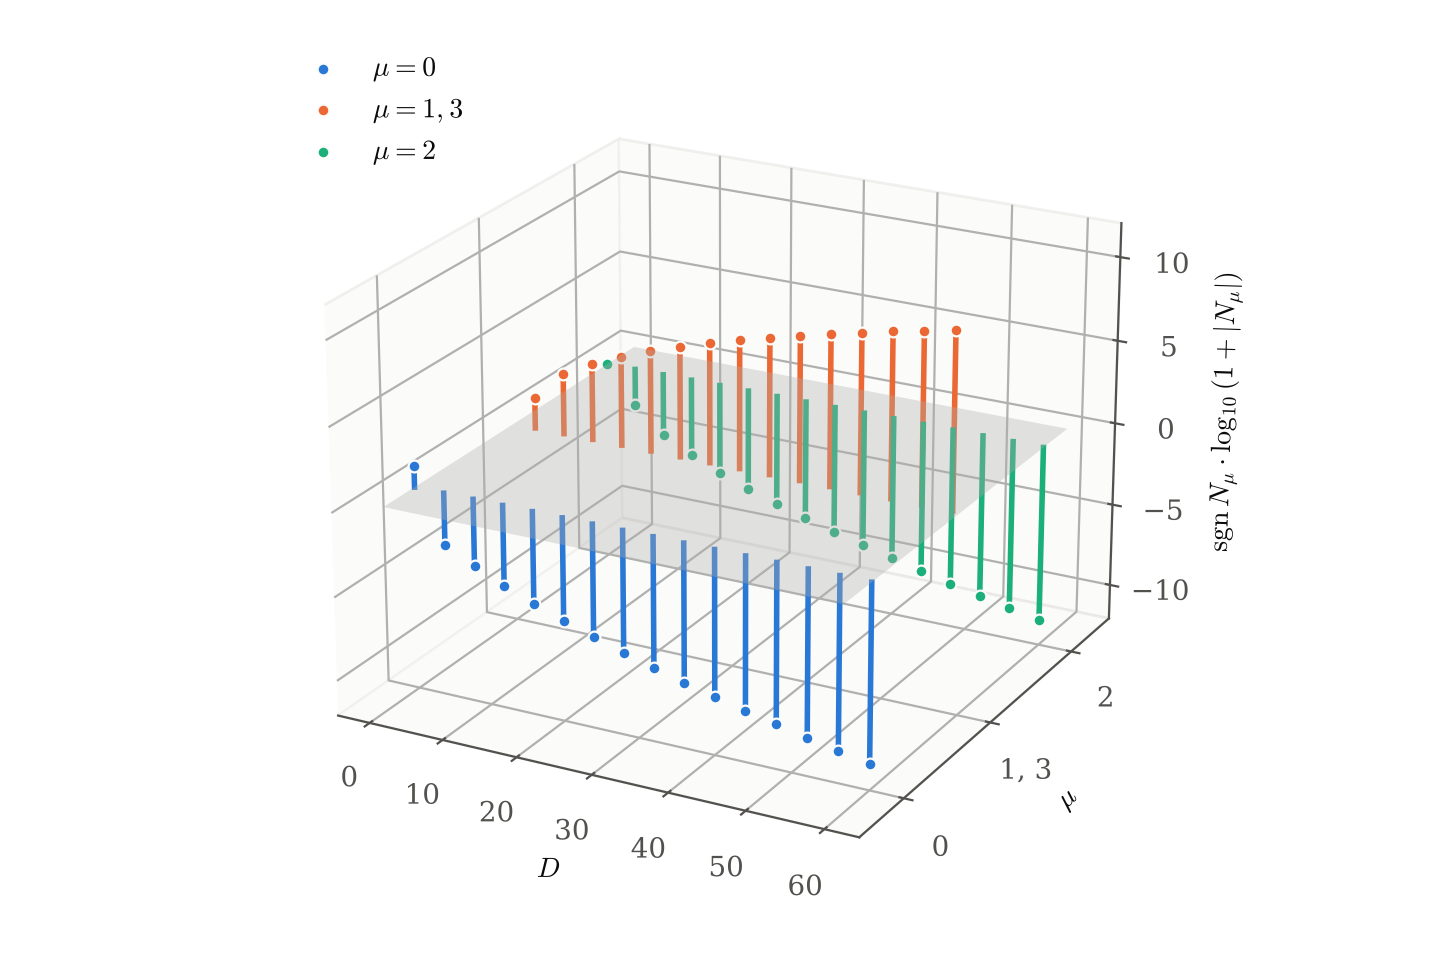
\includegraphics[width=0.78\textwidth]{fig_signs.png}
\caption{The coefficients $N_\mu(D)$ of the numerator of $\varphi^F_2$ for $0\le D\le60$, plotted as $\operatorname{sgn}N_\mu\cdot\log_{10}(1+|N_\mu|)$ over the plane $N=0$. The component $\mu=0$ is positive only at $D=0$, the component $\mu=2$ is never positive, and the odd components are always positive.}\label{fig:signs}
\end{figure}

\begin{theorem}\label{thm:Q2}
In the $\ZZ_2$ CHL model, $d^*(Q,P)>0$ for every charge with $Q^2=2$, $P^2>0$ and $2P^2>(Q\cdot P)^2$, and for every charge in the $\Gamma_1(2)$ orbit of such a charge.
\end{theorem}

\begin{proof}
By Lemma~\ref{lem:setA} and \eqref{eq:dstar}, $d^*=(-1)^{\ell+1}c^F_2(n,\ell)$, and $c^F_2$ is given by \eqref{eq:Q2coeff} with $D=4n-\ell^2>0$; every $\beta(j)$ is positive.

If $\ell$ is odd, then $D\equiv3\pmod4$, every argument $D+4-4j$ is $\equiv3\pmod 4$, every term is nonnegative by Lemma~\ref{lem:Q2signs}(i), (ii), and the term $j=0$ is $N_1(D+4)>0$. So $d^*=c^F_2>0$.

If $\ell\equiv2\pmod4$, then $D\equiv0\pmod4$, every term is $\le0$ by Lemma~\ref{lem:Q2signs}(i), (iii), and the term $j=0$ is $N_2(D+4)<0$ since $D+4\ge8$. So $d^*=-c^F_2>0$.

If $\ell\equiv0\pmod4$, write $D=4u$ with $u\ge1$. Then $-c^F_2$ is the coefficient of $x^{u+1}$ in $f\prod_r(1-x^r)^{-e_r}$, with $f=\sum_{t\ge0}\big(-N_0(4t)\big)x^t$. By Lemma~\ref{lem:Q2signs}(iv), $f/16=-1+\sum_{t\ge1}a_tx^t$ with $a_t\ge68>16$, and Lemma~\ref{lem:product} with $K=16$ gives $-c^F_2>0$, so $d^*>0$. The orbits follow from the $\Gamma_1(2)$ invariance of $d^*$.
\end{proof}

\section{Reduction to a fundamental set of charges}\label{sec:reduction}

From now on $m$ is arbitrary. This section shows that the sign of $d^*$ has to be checked only on charges with $m\le n$ and $0\le\ell\le m$, and proves Theorem~\ref{thm:bounded}.

\subsection{The Fricke symmetry of the product formula}
The duality group $\Gamma_1(2)$ acts on the charges by $(Q,P)\mapsto(aQ+bP,\,cQ+dP)$ with $\begin{psmallmatrix}a&b\\c&d\end{psmallmatrix}\in\Gamma_1(2)$, that is, $c$ even and $a,d$ odd \cite[(5.17)--(5.19)]{BSS25}. It does not exchange $Q^2$ with $P^2/2$. The product formula has, however, an extra symmetry that does.

\begin{lemma}\label{lem:fricke}
Let $E(A,B,j)=\sum_{s=0}^1(-1)^{sB}c^{(A\bmod2,\,s)}_{j\bmod2}(2AB-j^2)$ be the exponent of the factor $1-x^A\e(B\rho)y^j$ in \eqref{eq:product}, where $x=\e(\sigma/2)$ and $A=2k'$. Then $E(A,B,j)=E(B,A,j)$ for all $A,B\ge0$ and $j$. Consequently
\begin{equation}\label{eq:fricke}
\Phit_6(\rho,\sigma,v)=\Phit_6\big(\tfrac\sigma2,\,2\rho,\,v\big)
\end{equation}
as formal products.
\end{lemma}

\begin{proof}
If $A$ and $B$ have the same parity, the two sides are the same expression. Let $A$ be even and $B$ odd; then $2AB-j^2\equiv-j^2\pmod4$ and $AB/2\in\ZZ$, and
\[
E(A,B,j)=c^{(0,0)}(N)-c^{(0,1)}(N),\qquad E(B,A,j)=c^{(1,0)}(N)+c^{(1,1)}(N),\qquad N=2AB-j^2,
\]
both read off at an integral power of $q$. By \eqref{eq:genera},
\[
F^{(0,0)}-F^{(0,1)}=\tfrac23\pB-\tfrac23\pA\,\fE(\tau),\qquad F^{(1,0)}+F^{(1,1)}=\tfrac23\pB-\tfrac13\pA\big(\fE(\tfrac\tau2)+\fE(\tfrac{\tau+1}2)\big).
\]
Since $\fE(\tau)=1+24\sum\sigma_1^{\rm odd}(n)q^n$ and $\sigma^{\rm odd}_1(2k)=\sigma^{\rm odd}_1(k)$,
\[
\fE(\tfrac\tau2)+\fE(\tfrac{\tau+1}2)=2+48\sum_{k\ge1}\sigma_1^{\rm odd}(2k)q^k=2\fE(\tau),
\]
so $F^{(0,0)}-F^{(0,1)}=F^{(1,0)}+F^{(1,1)}$ identically, and the exponents agree. The prefactor $\e(\rho+\frac\sigma2+v)$ and the range $A,B\ge0$, $j<0$ if $A=B=0$, of the product are symmetric under $A\leftrightarrow B$, which gives \eqref{eq:fricke}.
\end{proof}

\begin{remark}
The substitution $(\rho,\sigma)\mapsto(\sigma/2,2\rho)$ is the action on the Siegel upper half-space of the Fricke involution of $\Gamma_0(2)$; Persson and Volpato showed that the CHL models with a geometric symmetry are self-dual under the corresponding Fricke S-duality \cite{PV15}, and \eqref{eq:fricke} is its shadow on the partition function. We use only the elementary statement of Lemma~\ref{lem:fricke}.
\end{remark}

\subsection{A chamber shared by both orientations}
For a charge $(m,n,\ell)$ and a point $(\rho_2,\sigma_2,v_2)$ of imaginary parts, let
\[
c(m,n,\ell;\rho_2,\sigma_2,v_2)=\int\frac{\e(-m\rho-n\frac\sigma2-\ell v)}{\Phit_6(\rho,\sigma,v)}\,d\rho_1\,d\sigma_1\,dv_1,
\]
the integral running over a period cell of the real parts. Sen showed \cite[\S4]{Sen07} that this number is locally constant in the imaginary parts and jumps only across the walls of marginal stability, which for the $\ZZ_2$ CHL model are the hyperplanes
\begin{equation}\label{eq:wallsSen}
j\,v_2+n_1\sigma_2-m_1\rho_2=0,\qquad j\ \text{odd},\quad m_1\in\ZZ,\quad n_1\in\tfrac12\ZZ,\quad m_1n_1=\tfrac{1-j^2}4,
\end{equation}
coming from the double zeros of $\Phit_6$ with vanishing coefficient of $\rho\sigma-v^2$.

\begin{lemma}\label{lem:chamber}
Let $\mathcal R=\{\rho_2,\sigma_2>0,\ 0<-v_2<\frac12\min(\rho_2,\frac{\sigma_2}2)\}$.
\begin{enumerate}
\item[(i)] $\mathcal R$ meets no wall \eqref{eq:wallsSen}, so $c_{\mathcal R}(m,n,\ell)=c(m,n,\ell;\rho_2,\sigma_2,v_2)$ does not depend on the point of $\mathcal R$.
\item[(ii)] $c_{\mathcal R}(m,n,\ell)=c_{\mathcal R}(n,m,\ell)$.
\item[(iii)] If $D=2mn-\ell^2>0$ and $0\le\ell\le2m$, then $c^F_m(n,\ell)=c_{\mathcal R}(m,n,\ell)$.
\end{enumerate}
\end{lemma}

\begin{proof}
(i) For $j=\pm1$ one of $m_1,n_1$ vanishes and the wall is $|v_2|=|n_1|\sigma_2$ with $|n_1|\ge\frac12$, or $|v_2|=|m_1|\rho_2$ with $|m_1|\ge1$, or $v_2=0$; none meets $\mathcal R$. For $|j|\ge3$ the product $m_1n_1$ is negative, so $|n_1\sigma_2-m_1\rho_2|=|n_1|\sigma_2+|m_1|\rho_2\ge2\sqrt{|m_1n_1|\sigma_2\rho_2}=\sqrt{j^2-1}\,\sqrt{\sigma_2\rho_2}$, while on $\mathcal R$
\[
|j\,v_2|<\tfrac{|j|}2\min(\rho_2,\tfrac{\sigma_2}2)\le\tfrac{|j|}{2\sqrt2}\sqrt{\rho_2\sigma_2}<\sqrt{j^2-1}\,\sqrt{\rho_2\sigma_2}.
\]
(ii) The substitution of Lemma~\ref{lem:fricke} maps $\mathcal R$ to itself and exchanges the roles of $m$ and $n$.

(iii) Let $\rho_2\to\infty$ inside $\mathcal R$ with $\sigma_2$ and $v_2$ fixed. The integral over $\rho_1$ picks out $\varphi_m$, and $c_{\mathcal R}(m,n,\ell)$ is the coefficient of $x^ny^\ell$ of $\varphi_m$ expanded in the strip $-\sigma_2<v_2<0$, where $|p|<|y|^{-1}<1$. Write $\varphi_m=\varphi^P_m+\varphi^F_m$ with \eqref{eq:polar}. The finite part is holomorphic in $v$, so its expansion does not depend on the strip. In the polar part, expand $\mathcal A_{2,m}$ in the strip: the term $s=0$ is $y(1-y)^{-2}=\sum_{k\ge1}k\,y^{-k}$, the terms $s\ge1$ contain only powers $y^{2ms+1+k}$ with $k\ge0$, and the terms $s\le-1$, rewritten through $(1-p^sy)^{-2}=p^{-2s}y^{-2}(1-p^{-s}y^{-1})^{-2}$, only powers $y^{2ms-1-k}$ with $k\ge0$. None of these exponents lies in $[0,2m]$, and the factor $1/g(\sigma/2)$ does not change the power of $y$. Hence the polar part contributes nothing at $y^\ell$ with $0\le\ell\le2m$.
\end{proof}

\subsection{Least representatives}
\begin{lemma}\label{lem:leastA}
Let $(m,n,\ell)$ be a charge with $m\ge1$, $|\ell|\le m$, $|\ell|\le n$ and $D=2mn-\ell^2>0$. Then it lies in the set $\mathcal A$ of \eqref{eq:setA}.
\end{lemma}

\begin{proof}
For $m_1=0$ the bracket in \eqref{eq:setA} is $m^2(2s+1)^2\ge m^2$. Let $m_1\ne0$, so $|m_1|\ge2$, and let $d$ be the distance from $m_1\ell$ to the nearest odd multiple of $m$; the bracket is at least $d^2+m_1^2D$. If $|m_1\ell|\le m$, then $d\ge m-|m_1\ell|$ and
\[
d^2+m_1^2D\ \ge\ m^2-2m|m_1\ell|+m_1^2\ell^2+m_1^2(2mn-\ell^2)=m^2+2m|m_1|\big(|m_1|n-|\ell|\big)\ \ge\ m^2 .
\]
If $|m_1\ell|>m$, then $D\ge2m|\ell|-\ell^2\ge m|\ell|$ and $m_1^2D\ge m|m_1|\cdot|m_1\ell|>2m^2$.
\end{proof}

\begin{definition}
A charge $(m,n,\ell)$ is \emph{reduced} if $1\le m\le n$, $0\le\ell\le m$ and $D=2mn-\ell^2>0$. For a reduced charge put $x=\sqrt D/m$ and $\theta=\pi\ell/m$. Since $D\ge2m^2-m^2$, every reduced charge has $x\ge1$.
\end{definition}

\begin{proposition}\label{prop:reduction}
For every charge $(Q,P)$ with $D>0$ there is a reduced charge $(m',n',\ell')$ with the same discriminant and $\ell'\equiv Q\cdot P\pmod2$ such that
\[
d^*(Q,P)=(-1)^{\ell'+1}c^F_{m'}(n',\ell')=(-1)^{\ell'+1}c_{\mathcal R}(m',n',\ell').
\]
\end{proposition}

\begin{proof}
In the orbit of $(Q,P)$ choose a charge with least $m=Q^2$; since $D>0$ the form $f(a,b)=(aQ+bP)^2=a^2m+2ab\ell+2b^2n$ is positive definite, so the least value exists. The matrices $\begin{psmallmatrix}1&0\\c&1\end{psmallmatrix}$ with $c$ even fix $Q$ and send $\ell$ to $\ell+cm$; so we may assume $|\ell|\le m$. The matrices $\begin{psmallmatrix}1&\pm1\\0&1\end{psmallmatrix}$ send $m$ to $m\pm2\ell+2n$, and minimality gives $n\ge|\ell|$. By Lemma~\ref{lem:leastA} the charge lies in $\mathcal A$, so $d^*=(-1)^{\ell+1}c^F_m(n,\ell)$ by \eqref{eq:dstar}. The finite part is a mock Jacobi form, even in $v$, so $c^F_m(n,\ell)=c^F_m(n,|\ell|)$. If $m\le n$, the charge $(m,n,|\ell|)$ is reduced. If $n<m$, then $0\le|\ell|\le n$ and Lemma~\ref{lem:chamber} gives $c^F_m(n,|\ell|)=c_{\mathcal R}(m,n,|\ell|)=c_{\mathcal R}(n,m,|\ell|)=c^F_n(m,|\ell|)$, and $(n,m,|\ell|)$ is reduced. The shifts change $\ell$ by even multiples of $m$ and the sign change does not alter the parity, so $\ell'\equiv Q\cdot P\pmod2$.
\end{proof}

So for the rest of the paper we write $d^*(m,n,\ell)=(-1)^{\ell+1}c^F_m(n,\ell)$ for a reduced charge, and the conjecture is the statement $d^*(m,n,\ell)>0$ on reduced charges.

\subsection{Bounded discriminant}
\begin{proof}[Proof of Theorem~\textup{\ref{thm:bounded}}]
A reduced charge with $D\le\Dexact$ has $m\le\sqrt D\le\lfloor\sqrt{\Dexact}\rfloor$ and $n=(D+\ell^2)/2m\le(D+m^2)/2m$, so there are finitely many. For each $\Gamma_1(2)$ orbit with $D\le\Dexact$ the program of Appendix~\ref{app:exact} finds a charge of least $Q^2$ satisfying \eqref{eq:setA} with $0\le\ell<2m$, and computes $c_{\mathcal R}(m,n,\ell)$ exactly from the product formula, in the cheaper of the two orientations allowed by Lemma~\ref{lem:chamber}. For $D\le\Dexact$ there are $\Norbits$ orbits; in every one of them $(-1)^{\ell+1}c_{\mathcal R}(m,n,\ell)>0$. By Lemma~\ref{lem:chamber}(iii) and \eqref{eq:dstar} these numbers are the single-centred indices.\footnote{Every orbit is found with all its representatives inside the computed box, and the program checks that they give the same value; at $Q^2=1,2$ it reproduces the closed formulas of Propositions~\ref{prop:Q1closed} and~\ref{prop:Q2closed}.}
\end{proof}

\section{Farey walls}\label{sec:walls}

The polar coefficients that enter the Rademacher series are sums over matrices of $SL_2(\ZZ)$ attached to Farey intervals, the continued-fraction walls of \cite{CNR21,CV08}. This section collects the elementary facts about them that the estimates need.

\subsection{The walls of a polar term}
Fix $m\ge1$, $\nu\in\frac12\ZZ$ and $\tilde\ell\in\ZZ$ with $0\le\tilde\ell<2m$ and
\[
\tilde D=4m\nu-\tilde\ell^2<0,\qquad t=-\tilde D,\qquad \omega_0=\frac{\tilde\ell}{2m},\qquad \delta=\frac{\sqrt t}{2m}.
\]
Let $\mathcal W(m,\nu,\tilde\ell)$ be the set of $G=\begin{psmallmatrix}p&q\\r&s\end{psmallmatrix}\in SL_2(\ZZ)$ with $r,s\ge1$ and $q/s\le\omega_0<p/r$; for each such $G$ put
\begin{equation}\label{eq:mGnG}
m_G=r^2\nu+p^2m-pr\tilde\ell,\qquad n_G=s^2\nu+q^2m-qs\tilde\ell,\qquad \ell_G=-2rs\nu-2pqm+(ps+qr)\tilde\ell .
\end{equation}
These are the coefficients of the quadratic form $\phi(X,Y)=\nu X^2-\tilde\ell XY+mY^2$ transformed by $G$: $m_G=\phi(r,p)$, $n_G=\phi(s,q)$, and $\ell_G$ is the cross term up to sign.

\begin{lemma}\label{lem:walls}
Let $G\in\mathcal W(m,\nu,\tilde\ell)$ and $U=p/r-\omega_0$, $W=\omega_0-q/s$, so that $U>0$, $W\ge0$ and $U+W=1/rs$.
\begin{enumerate}
\item[(i)] $\ell_G^2-4m_Gn_G=t$.
\item[(ii)] $m_G=mr^2(U^2-\delta^2)$, $n_G=ms^2(W^2-\delta^2)$, $\ell_G=2mrs(UW+\delta^2)>0$, and $m=m_Gs^2+n_Gr^2+\ell_Grs$.
\item[(iii)] $E_G:=m-m_G-n_G-\ell_G=m\big[1-(rU+sW)^2+\delta^2(r-s)^2\big]\ge0$.
\item[(iv)] If $m_G,n_G\ge-1$, put $a=m_G$, $b=n_G$, $S=a+b+2$ and $t_0=m^2+4m$. Then
\begin{equation}\label{eq:t0t}
t_0-t=S(2m-S)+E_G^2+2E_G\ell_G+4(a+1)(b+1),
\end{equation}
so $t\le t_0$; moreover $t_0-t\le2mS$ when $r=s=1$.
\item[(v)] If $m_G,n_G\ge-1$, then $a\le m/s^2$, $b\le m/r^2$ and $r,s\le2m$.
\item[(vi)] If $m_G,n_G\ge-1$ and $rs\ge2$, then $\delta\le\frac14+\frac5{2m}$, that is $\sqrt t\le\frac m2+5$.
\item[(vii)] If $r=s=1$, then $G=\begin{psmallmatrix}1&0\\1&1\end{psmallmatrix}$, $a=\nu+m-\tilde\ell$, $b=\nu$, $\ell_G=m-a-b$, $E_G=0$ and $\tilde\ell=m+b-a$. Conversely every pair $(a,b)$ of integers with $a,b\ge-1$, $k:=m-a-b\ge1$, $t=k^2-4ab>0$ and $-m\le b-a<m$ arises from exactly one polar term with $\nu=b\in\ZZ$ in this way.
\end{enumerate}
\end{lemma}

\begin{proof}
(i) $\phi\circ G$ has the same discriminant as $\phi$. (ii) $\phi(r,p)=r^2\big(\nu-\tilde\ell u+mu^2\big)$ with $u=p/r$, and $\nu-\tilde\ell u+mu^2=m\big((u-\omega_0)^2-\delta^2\big)$ because $\tilde\ell^2-4m\nu=4m^2\delta^2$; similarly for $n_G$. For $\ell_G$ write $\ell_G=2mrs\big[(p/r-\omega_0)(\omega_0-q/s)+\delta^2\big]$, which is \eqref{eq:mGnG} after expanding and using $ps-qr=1$. The last identity follows from $\phi(r,p)s^2+\phi(s,q)r^2+\ell_Grs=m(ps-qr)^2$. (iii) Insert (ii) in the definition and use $U+W=1/rs$; then $rU+sW\le\max(r,s)(U+W)=1/\min(r,s)\le1$. (iv) By (i), $t=\ell_G^2-4ab$ with $\ell_G=m-a-b-E_G=m+2-S-E_G$; expand $t_0-t=m^2+4m-(m+2-S-E_G)^2+4ab$ and use $4ab=4(a+1)(b+1)-4S+4$. For $r=s=1$, $E_G=0$ and $4(a+1)(b+1)\le S^2$. (v) $a=mr^2(U^2-\delta^2)\le mr^2U^2\le m/s^2$, and $b\le m/r^2$ in the same way. Since $t\ge1$, $\delta\ge1/2m$. From $a\ge-1$, $\delta^2\le U^2+1/(mr^2)$, and from $b\ge-1$, $\delta^2\le W^2+1/(ms^2)$. One of $U,W$ is at most $1/(2rs)$; if it is $U$, the first inequality gives $r^2\le4m^2(\frac1{4s^2}+\frac1m)\le m^2+4m$, so $r\le m+1$, and the second with $W\le1/rs$ gives $s^2\le4m^2(1+\frac1m)$, so $s\le2m$. The other case is symmetric. (vi) If $\delta\le\frac14$ there is nothing to prove. Otherwise, from $a\ge-1$, $\delta-U\le1/(mr^2(\delta+U))\le4/(mr^2)$, and from $b\ge-1$, $\delta-W\le4/(ms^2)$. Adding, $2\delta\le\frac1{rs}+\frac4m\big(\frac1{r^2}+\frac1{s^2}\big)\le\frac12+\frac5m$ when $rs\ge2$. (vii) $p-q=1$ and $q\le\omega_0<q+1$ with $0\le\omega_0<1$ force $q=0$, $p=1$. The formulas follow from \eqref{eq:mGnG}. Given $(a,b)$, put $\nu=b$ and $\tilde\ell=m+b-a\in[0,2m)$; then $\tilde D=4mb-(m+b-a)^2=-(k^2-4ab)$.
\end{proof}

\begin{remark}
\begin{figure}[t]
\centering
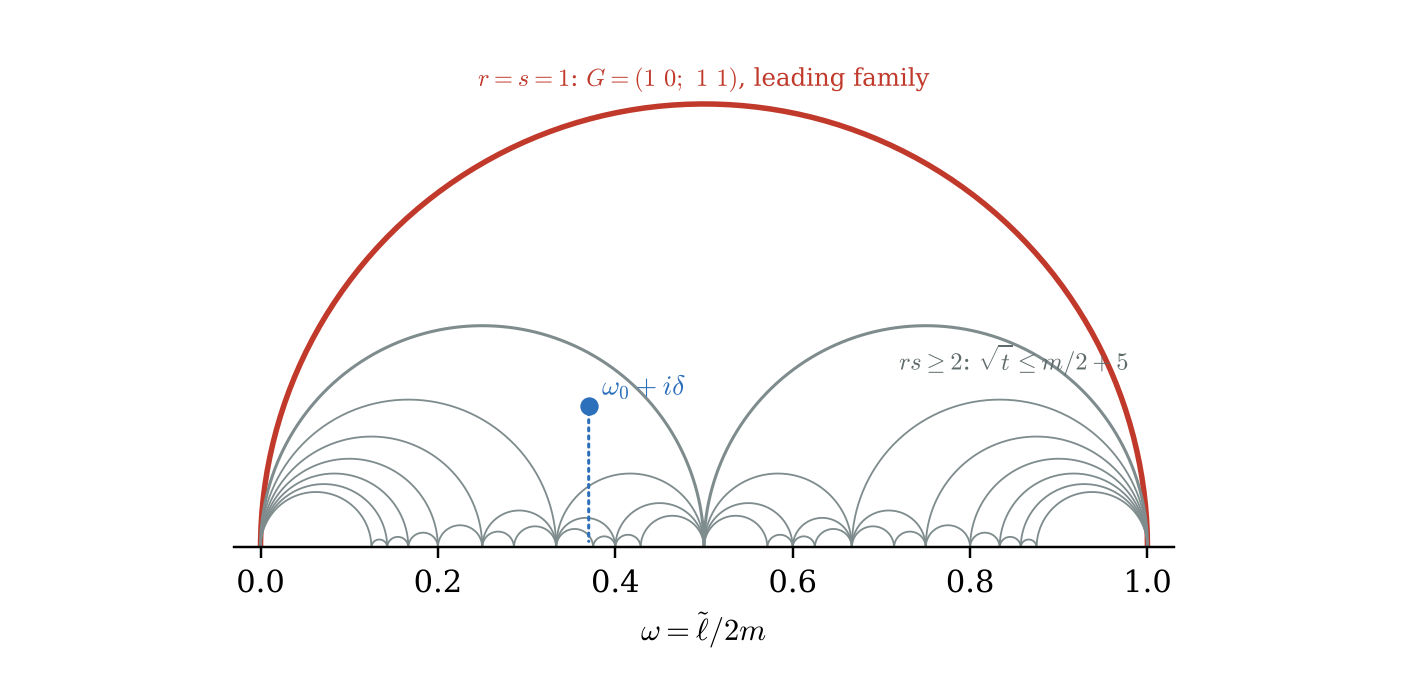
\includegraphics[width=0.86\textwidth]{fig_walls.png}
\caption{The Farey walls of a polar term at the cusp $0$, drawn as geodesics from $q/s$ to $p/r$ in the upper half-plane of $\omega=\tilde\ell/2m$. A matrix $G=\begin{psmallmatrix}p&q\\r&s\end{psmallmatrix}$ contributes to the polar coefficient at $(\tilde\ell,\nu)$ when its geodesic passes over the point $\omega_0+i\delta$ with $\omega_0=\tilde\ell/2m$ and $\delta=\sqrt{-\tilde D}/2m$ (Lemma~\ref{lem:walls}). The outer red geodesic is the leading family $r=s=1$; every other wall lies below height $\frac14+\frac5{2m}$.}\label{fig:wallsfig}
\end{figure}

Lemma~\ref{lem:walls}(iii) is the reason why the leading family dominates: by \eqref{eq:t0t} the walls with $r=s=1$ are exactly those for which $t_0-t$ is as small as the pair $(a,b)$ allows, and by (vi) every other wall has $\sqrt t$ at most about half of $\sqrt{t_0}$. Figure~\ref{fig:wallsfig} shows the geometry.
\end{remark}

\subsection{Polar coefficients}
Let $d_1(k)$, $k\ge-1$, be the coefficients of
\begin{equation}\label{eq:d1}
\frac1{\eta(\tau)^8\eta(2\tau)^8}=\sum_{k\ge-1}d_1(k)\,q^k=q^{-1}+8+52q+256q^2+1122q^3+\cdots,
\end{equation}
so that $d_1(k)=\hat f(k)$ in the notation of \eqref{eq:polar}, and put $d_1(k)=0$ unless $k\ge-1$ is an integer. For a polar term $(\nu,\tilde\ell)$ define
\begin{align}
a_S(\nu,\tilde\ell)&=\frac1{16}\sum_{G\in\mathcal W(m,\nu,\tilde\ell)}\ell_G\,d_1(m_G)\,d_1(n_G)\qquad(\nu\in\ZZ),\label{eq:P0}\\
a_I(\nu,\tilde\ell)&=\sum_{G\in\mathcal W(m,\nu,\tilde\ell)}\ell_G\Big([r\ \text{even}]\,d_1(m_G)\,d_1(2n_G)+[s\ \text{even}]\,d_1(2m_G)\,d_1(n_G)\Big)\qquad(\nu\in\tfrac12\ZZ),\label{eq:Pinf}
\end{align}
and $a_T(\nu,\tilde\ell)=(-1)^{2\nu}a_I(\nu,\tilde\ell)$. The sums are finite by Lemma~\ref{lem:walls}(v). Formula \eqref{eq:P0} is the continued-fraction formula of \cite[(2.43)]{CNR21} for $1/\Phi_{10}$ with the coefficients of $1/\eta^{24}$ replaced by $d_1$ and with no congruence condition on $G$, and \eqref{eq:Pinf} is its parity-restricted form \cite[(4.21)]{CNR21}.\footnote{In \eqref{eq:Pinf} the condition that $r$ or $s$ be even selects the walls that are images of the basic wall under $\Gamma_0(2)$ or its conjugate; the factor $d_1(2n_G)$ vanishes unless $2n_G$ is an integer.}

\section{The level-two Rademacher expansion}\label{sec:hypothesis}

This section states the one input of Theorem~\ref{thm:all} that is not proved here, explains where it comes from, and records the evidence for it.

\subsection{Frames and Weil sums}
Let $\Gamma^0(2)$ be the group of matrices of $SL_2(\ZZ)$ with even upper right entry. It has index three, and
\[
R_I=\begin{pmatrix}1&0\\0&1\end{pmatrix},\qquad R_T=\begin{pmatrix}1&1\\0&1\end{pmatrix},\qquad R_S=\begin{pmatrix}0&-1\\1&0\end{pmatrix}
\]
represent its right cosets. For $M\in SL_2(\ZZ)$ the \emph{frame} of $M$ is the $F\in\{I,T,S\}$ with $MR_F^{-1}\in\Gamma^0(2)$. The three frames correspond to the expansions of a form for $\Gamma^0(2)$ at the cusp $\infty$ (frames $I$ and $T$, which differ by a half period) and at the cusp $0$ (frame $S$).\footnote{The duality group $\Gamma_1(2)$ acts on the charges; the finite part $\varphi^F_m(\sigma,v)$ is a function of $\sigma$ on which the relevant group, after the substitution $x=\e(\sigma/2)$, is $\Gamma^0(2)$. The cusp $\infty$ has width two, which is why it carries two frames.}

For $\gamma\ge1$ let $\mathcal C_\gamma$ be the set of pairs $(\gamma,\delta)$ with $-\delta\in\{0,1,\dots,2\gamma-1\}$ and $\gcd(\gamma,\delta)=1$. For each such pair let $\alpha\in\{0,\dots,\gamma-1\}$ be the inverse of $\delta$ modulo $\gamma$ (with $\alpha=0$ if $\gamma=1$), let $\beta=(\alpha\delta-1)/\gamma$, and let $F(\gamma,\delta)$ be the frame of $\begin{psmallmatrix}\delta&-\beta\\-\gamma&\alpha\end{psmallmatrix}$. For $\tilde\ell,\ell\in\ZZ$ put
\begin{equation}\label{eq:weil}
W_{\gamma,\delta}(\tilde\ell,\ell)=\frac1{\sqrt{2m\gamma i}}\sum_{T=0}^{\gamma-1}\e\Big(\frac{\alpha x^2-2\ell x+\delta\ell^2}{4m\gamma}\Big),\qquad x=\tilde\ell-2mT,
\end{equation}
with the principal square root. This is the matrix coefficient of the Weil representation attached to the lattice $\sqrt{2m}\,\ZZ$, evaluated on the inverse of $\begin{psmallmatrix}\alpha&\beta\\\gamma&\delta\end{psmallmatrix}$ \cite[(2.41)]{CNR21}; it depends on $\tilde\ell$ only modulo $2m$.

\begin{lemma}\label{lem:weilbound}
$|W_{1,\delta}|=(2m)^{-1/2}$, and $|W_{\gamma,\delta}(\tilde\ell,\ell)|\le\sqrt{\gcd(m,\gamma)/m}$ for every $\gamma\ge1$.
\end{lemma}

\begin{proof}
For $\gamma=1$ the sum has one term. In general, $\alpha x^2/(4m\gamma)=\alpha\tilde\ell^2/(4m\gamma)-\alpha\tilde\ell T/\gamma+\alpha mT^2/\gamma$, so up to a factor of modulus one the sum is $\sum_{T\bmod\gamma}\e\big((\alpha mT^2+bT)/\gamma\big)$ for an integer $b$. A quadratic Gauss sum modulo $\gamma$ with leading coefficient $\alpha m$, $\gcd(\alpha,\gamma)=1$, has modulus at most $\sqrt{2\gcd(m,\gamma)\gamma}$ \cite[Chapter~1]{BEW98}. Dividing by $\sqrt{2m\gamma}$ gives the claim.
\end{proof}

\subsection{Polar data and shadows}
For $m\ge1$ the polar terms in each frame are the pairs $(\tilde\nu,\tilde\ell)$ with $0\le\tilde\ell<2m$ and $\tilde D=4m\tilde\nu-\tilde\ell^2<0$, where $\tilde\nu\in\ZZ$ in frame $S$ and $\tilde\nu\in\frac12\ZZ$ in frames $I$ and $T$. Their coefficients are the wall sums of Section~\ref{sec:walls}:
\begin{equation}\label{eq:polardata}
a_S(\tilde\nu,\tilde\ell)\ \text{from \eqref{eq:P0}},\qquad a_I(\tilde\nu,\tilde\ell)\ \text{from \eqref{eq:Pinf}},\qquad a_T(\tilde\nu,\tilde\ell)=(-1)^{2\tilde\nu}a_I(\tilde\nu,\tilde\ell).
\end{equation}
By Lemma~\ref{lem:walls}(iv) a wall with $m_G,n_G\ge-1$ has $t\le t_0=m^2+4m$, so only finitely many polar terms have a nonzero coefficient.

The shadow of the finite part is governed by the coefficient $\hat f(m)=d_1(m)$ of the polar part \eqref{eq:polar}. In the three frames it enters with the constants and the orders
\begin{equation}\label{eq:mockdata}
(c_S,\mu_S)=\big(\tfrac{1}{16}\hat f(m),\,1\big),\qquad (c_I,\mu_I)=\big(\hat f(m),\,\tfrac12\big),\qquad (c_T,\mu_T)=\big(-\hat f(m),\,\tfrac12\big).
\end{equation}
The number $\mu_F$ is the order of the pole of $1/g(\sigma/2)$ in the local parameter of the frame: $1/g$ has the term $x^{-1}=\e(-\sigma/2)$ at $\infty$, and its transform under $\sigma\mapsto-1/\sigma$ starts with $\e(-\sigma)/16$, by $\eta(-1/\tau)=\sqrt{-i\tau}\,\eta(\tau)$.\footnote{With $\tau=\sigma/2$, the substitution $\sigma\mapsto-1/\sigma$ is $\tau\mapsto-1/4\tau$, and $g(-1/4\tau)=\eta(-1/4\tau)^8\eta(-1/2\tau)^8=2^{12}\tau^8\eta(\sigma)^8\eta(2\sigma)^8$, whose expansion starts with $\e(\sigma)$.} For $\gamma\ge1$, $(\gamma,\delta)\in\mathcal C_\gamma$ and $g\in\ZZ$ put
\[
f_{\gamma,g}(u)=\begin{cases}\dfrac{\pi^2}{\sinh^2\!\big(\frac{\pi u}{\gamma}-\frac{i\pi g}{2m\gamma}\big)},& 2m\gamma\nmid g,\\[2.2ex]
\dfrac{\pi^2}{\sinh^2(\pi u/\gamma)}-\dfrac{\gamma^2}{u^2},& 2m\gamma\mid g.\end{cases}
\]

\subsection{The hypothesis}
For a charge $(m,n,\ell)$ with $m\ge1$, $0\le\ell\le m$ and $D=2mn-\ell^2>0$ define
\begin{align}
\mathcal M(m,n,\ell)&=\sum_{\gamma\ge1}\sum_{(\gamma,\delta)\in\mathcal C_\gamma}\ \sum_{(\tilde\nu,\tilde\ell)}a_{F}(\tilde\nu,\tilde\ell)\,\e\Big(\frac{\alpha\tilde D+\delta D}{4m\gamma}\Big)W_{\gamma,\delta}(\tilde\ell,\ell)\,\frac{2\pi}\gamma\Big(\frac{|\tilde D|}{D}\Big)^{\frac{15}4}I_{\frac{15}2}\Big(\frac{\pi\sqrt{|\tilde D|D}}{m\gamma}\Big),\label{eq:radmain}\\
\mathcal K_2(m,n,\ell)&=-\sqrt{2m}\sum_{\gamma\ge1}\gamma^{-\frac12}\!\!\sum_{(\gamma,\delta)\in\mathcal C_\gamma}\!\! c_F\,\e\Big(\frac{-4m\mu_F\alpha+\delta D}{4m\gamma}\Big)W_{\gamma,\delta}(0,\ell)\Big(\frac{4m\mu_F}{D}\Big)^4I_8\Big(\frac{2\pi}\gamma\sqrt{\frac{\mu_FD}m}\Big),\label{eq:radK2}\\
\mathcal K_3(m,n,\ell)&=\frac1{2\pi}\sum_{\gamma\ge1}\gamma^{-2}\!\!\sum_{(\gamma,\delta)\in\mathcal C_\gamma}\ \sum_{g=-m\gamma}^{m\gamma-1}c_F\,\e\Big(\frac{-\alpha(4m\mu_F+g^2)+\delta D}{4m\gamma}\Big)W_{\gamma,\delta}(g,\ell)\Big(\frac{4m\mu_F}{D}\Big)^{\frac{17}4}\label{eq:radK3}\\
&\qquad\times\int_{-\sqrt{\mu_F/m}}^{\sqrt{\mu_F/m}}f_{\gamma,g}(u)\Big(1-\frac{mu^2}{\mu_F}\Big)^{\frac{17}4}I_{\frac{17}2}\Big(\frac{2\pi}\gamma\sqrt{\frac{(\mu_F-mu^2)D}m}\Big)\,du,\notag
\end{align}
where in each line $F=F(\gamma,\delta)$ and $\alpha,\beta$ are attached to $(\gamma,\delta)$ as above.

\begin{hypothesis}\label{hyp:R}
For every charge $(m,n,\ell)$ with $m\ge1$, $0\le\ell\le m$ and $D=2mn-\ell^2>0$,
\begin{equation}\label{eq:hypR}
(-1)^{\ell+1}c^F_m(n,\ell)=\tfrac12(-1)^\ell\sqrt i\,\big(\mathcal M+\mathcal K_2+\mathcal K_3\big)(m,n,\ell).
\end{equation}
\end{hypothesis}

\begin{lemma}\label{lem:radconv}
The three series \eqref{eq:radmain}--\eqref{eq:radK3} converge absolutely.
\end{lemma}

\begin{proof}
There are at most $2\gamma$ pairs in $\mathcal C_\gamma$, the polar terms are finitely many, and $|W|\le1$ by Lemma~\ref{lem:weilbound}. Since $I_\nu(z)/z^\nu$ is increasing, $I_\nu(z/\gamma)\le\gamma^{-\nu}I_\nu(z)$ for $\gamma\ge1$. So the $\gamma$-th term of \eqref{eq:radmain} is $O(\gamma\cdot\gamma^{-1}\cdot\gamma^{-15/2})$, that of \eqref{eq:radK2} is $O(\gamma^{1-1/2-8})$. In \eqref{eq:radK3}, for $2m\gamma\nmid g$ one has $|\sinh(a-ib)|^2=\sinh^2a+\sin^2b\ge\sin^2b$, so $|f_{\gamma,g}|\le\pi^2\csc^2(\pi g/2m\gamma)$, and for $g=0$ the function $\pi^2/\sinh^2y-\pi^2/y^2$ takes values in $[-\pi^2/3,0)$. With the identity $\sum_{g=1}^{N-1}\csc^2(\pi g/N)=(N^2-1)/3$ for $N=2m\gamma$,
\begin{equation}\label{eq:fsum}
\sum_{g=-m\gamma}^{m\gamma-1}\sup_u|f_{\gamma,g}(u)|\le\frac{\pi^2(4m^2\gamma^2-1)}3+\frac{\pi^2}3=\frac{4\pi^2m^2\gamma^2}3,
\end{equation}
so the $\gamma$-th term of \eqref{eq:radK3} is $O(\gamma\cdot\gamma^{-2}\cdot\gamma^2\cdot\gamma^{-17/2})$. Only absolute bounds are used below, except for the terms with $\gamma=1$ in frame $S$, which are computed explicitly in Section~\ref{sec:model}.
\end{proof}

\begin{remark}\label{rem:hypsource}
Hypothesis~\ref{hyp:R} has three ingredients.
\begin{enumerate}
\item[(H)] The shape of the expansion: a mixed mock Jacobi form of weight $-6$ and index $m$ for $\Gamma^0(2)$, whose shadow is a multiple of the vector of unary theta functions of index $m$ with coefficient $1/g$, has Fourier coefficients given by the vector-valued Rademacher series over the three frames, with the main Bessel terms $I_{15/2}$ from the principal parts and the correction terms $I_8$ and $I_{17/2}$ from the shadow. For a weakly holomorphic Jacobi form at level $N$ this is the classical circle method of Rademacher and Zuckerman \cite{RZ38,Zuc39}, written for Jacobi forms by its theta decomposition. For mixed mock Jacobi forms on $SL_2(\ZZ)$, which is the case of $1/\Phi_{10}$, the expansion was proved by Bringmann and Manschot \cite{BMa13} and used by Ferrari and Reys \cite{FR17}; the correction terms come from the non-holomorphic completion of Zwegers \cite{Zwe02}. At level two it is stated in \cite[\S4]{CNR21}, where it is assumed in the derivation of the immortal index, and we do not know a proof.
\item[(P0)] The principal part at the cusp $0$ is given by the wall sum \eqref{eq:P0}: the continued-fraction formula of \cite[(2.43)]{CNR21} with $d_1$ in place of the coefficients of $1/\eta^{24}$.
\item[(P$\infty$)] The principal part at the cusp $\infty$ is given by the parity-restricted wall sum \eqref{eq:Pinf}.
\end{enumerate}
The constants \eqref{eq:mockdata} are part of (H): they are the shadow coefficients of $\varphi^F_m$ in the three frames, read off from the polar part \eqref{eq:polar}, whose shadow is the image of $\hat f(m)\mathcal A_{2,m}/g$ under the completion of the Appell--Lerch sum \cite{Zwe02,DMZ12}.
\end{remark}

\subsection{Evidence}\label{ssec:evidence}
We have tested the three ingredients separately and together.
\begin{enumerate}
\item[(a)] For $m=1,2$ the coefficients $c^F_m(n,\ell)$ are known in closed form (Propositions~\ref{prop:Q1closed} and~\ref{prop:Q2closed}). The right side of \eqref{eq:hypR}, truncated at $\gamma\le8$ in $\mathcal M$ and at $\gamma\le4$ in $\mathcal K_2$ and $\mathcal K_3$, agrees with them to relative precision $10^{-21}$ for every $n\le42$.
\item[(b)] For $m=3$ ($n=8,12$) and $m=4$ ($n=10,12$), with the same truncation ($\gamma\le8$ in $\mathcal M$, $\gamma\le4$ in $\mathcal K_2,\mathcal K_3$) and with $c^F_m(n,\ell)$ computed exactly from the product formula, the relative difference is below $10^{-13}$ for every $0\le\ell\le m$. The size of the omitted terms, estimated by Lemma~\ref{lem:radconv}, is of the same order, so the agreement is as good as the truncation allows.
\item[(c)] The polar coefficients at the cusp $\infty$ are Fourier coefficients of $\varphi^F_m$ itself, computable from the product formula. On all $373$ polar terms with $m\le14$ they agree with \eqref{eq:Pinf}.
\item[(d)] The polar coefficients at the cusp $0$ can be computed by expanding $\varphi_m$ at that cusp, where the twisted genera \eqref{eq:genera} are permuted by $\sigma\mapsto-1/\sigma$, and subtracting the transform of the polar part. On all $168$ polar terms with $m\le10$ they agree with \eqref{eq:P0}.
\end{enumerate}
All of these are exact or high-precision computations; the programs are in the archive \cite{Bha26c}.

\begin{remark}
Without (P0) and (P$\infty$), (H) alone would still give an expansion whose principal parts are \emph{some} finite sets of numbers. What the proof of Theorem~\ref{thm:all} uses from (P0) is exactly the structure of Lemma~\ref{lem:walls}: the leading family of walls and the bound (vi) for the others. From (P$\infty$) it uses only that every wall in it has $r$ or $s$ even, hence $rs\ge2$, so that Lemma~\ref{lem:walls}(vi) applies.
\end{remark}

\section{The leading family and an eta quotient}\label{sec:model}

Fix $m\ge1$ and a charge $(m,n,\ell)$ with $0\le\ell\le m$ and $D>0$; write $x=\sqrt D/m$, $\theta=\pi\ell/m$ and $t_0=m^2+4m$. The \emph{extreme term} is
\begin{equation}\label{eq:ext}
\mathcal E(D,m)=\frac{\pi}{\sqrt{2m}}\cdot\frac{m+2}{16}\Big(\frac{t_0}D\Big)^{\frac{15}4}I_{\frac{15}2}\big(\pi x\sqrt{t_0}\big)>0 .
\end{equation}
It is the contribution to $\frac12(-1)^\ell\sqrt i\,\mathcal M$ of the frame $S$, $\gamma=1$, and the most polar term $\tilde\nu=-1$, $\tilde\ell=m$, whose only wall is $G_0=\begin{psmallmatrix}1&0\\1&1\end{psmallmatrix}$ with $m_{G_0}=n_{G_0}=-1$ and $\ell_{G_0}=m+2$.

\subsection{The terms with \texorpdfstring{$\gamma=1$}{gamma=1}}
For $\gamma=1$ the set $\mathcal C_1$ consists of $\delta=0$ and $\delta=-1$, both with $\alpha=0$ and $\beta=-1$. The matrix $\begin{psmallmatrix}0&1\\-1&0\end{psmallmatrix}$ has frame $S$, and $\begin{psmallmatrix}-1&1\\-1&0\end{psmallmatrix}$ has frame $T$. So the terms with $\gamma=1$ are one term in frame $S$ and one in frame $T$.

In frame $S$, $W_{1,0}(\tilde\ell,\ell)=(2mi)^{-1/2}\e(-\ell\tilde\ell/2m)$ and the phase in \eqref{eq:radmain} is $1$. Since $\sqrt i/\sqrt{2mi}=1/\sqrt{2m}$,
\begin{equation}\label{eq:gamma1S}
\tfrac12(-1)^\ell\sqrt i\,\mathcal M_{\gamma=1,S}=\frac{\pi}{\sqrt{2m}}\sum_{(\tilde\nu,\tilde\ell)}a_S(\tilde\nu,\tilde\ell)\,(-1)^\ell\e\Big(-\frac{\ell\tilde\ell}{2m}\Big)\Big(\frac tD\Big)^{\frac{15}4}I_{\frac{15}2}(\pi x\sqrt t),\qquad t=-\tilde D .
\end{equation}
Split $a_S=a_S^{\rm lead}+a_S^{\rm rest}$, where $a_S^{\rm lead}$ is the term of $G_0$ in \eqref{eq:P0} and $a_S^{\rm rest}$ the sum over the walls with $rs\ge2$. Lemma~\ref{lem:walls}(vii) identifies the polar terms carrying $G_0$ with the set
\[
\mathcal L_m=\big\{(a,b)\in\ZZ^2:\ a,b\ge-1,\ k=m-a-b\ge1,\ t_{a,b}=k^2-4ab>0,\ -m\le b-a<m\big\},
\]
by $\tilde\nu=b$, $\tilde\ell=m+b-a$, with $a_S^{\rm lead}=\frac1{16}k\,d_1(a)d_1(b)$ and $t=t_{a,b}$. For $(a,b)\in\mathcal L_m$ put $S=a+b+2$ and
\begin{equation}\label{eq:rho}
\rho_{a,b}(x)=\frac{k}{m+2}\Big(\frac{t_{a,b}}{t_0}\Big)^{\frac{15}4}\frac{I_{15/2}(\pi x\sqrt{t_{a,b}})}{I_{15/2}(\pi x\sqrt{t_0})}.
\end{equation}

\begin{theorem}\label{thm:model}
The leading part of \eqref{eq:gamma1S} is
\begin{equation}\label{eq:leadsum}
\begin{split}
&\frac{\pi}{\sqrt{2m}}\sum_{(\tilde\nu,\tilde\ell)}a^{\rm lead}_S(\tilde\nu,\tilde\ell)\,(-1)^\ell\e\Big(-\frac{\ell\tilde\ell}{2m}\Big)\Big(\frac tD\Big)^{\frac{15}4}I_{\frac{15}2}(\pi x\sqrt t)\\
&\qquad=\mathcal E(D,m)\sum_{(a,b)\in\mathcal L_m}d_1(a)d_1(b)\,\rho_{a,b}(x)\cos\big((a-b)\theta\big).
\end{split}
\end{equation}
Moreover $\rho_{-1,-1}=1$, and with $z=e^{-\pi x+i\theta}$,
\begin{equation}\label{eq:modelsum}
\sum_{a,b\ge-1}d_1(a)d_1(b)\,e^{-\pi x(a+b+2)}\cos\big((a-b)\theta\big)=|P(z)|^2,\qquad P(z)=\prod_{n\ge1}(1-z^n)^{-8}(1-z^{2n})^{-8}.
\end{equation}
\end{theorem}

\begin{proof}
With $\tilde\ell=m+b-a$ one has $(-1)^\ell\e(-\ell\tilde\ell/2m)=(-1)^\ell(-1)^\ell\e(\ell(a-b)/2m)=e^{i(a-b)\theta}$. Dividing the term of $(a,b)$ by $\mathcal E(D,m)$ leaves $d_1(a)d_1(b)\rho_{a,b}(x)e^{i(a-b)\theta}$. The conditions defining $\mathcal L_m$ other than $-m\le b-a<m$ are symmetric in $(a,b)$, and the weight $d_1(a)d_1(b)\rho_{a,b}$ is symmetric; so the terms of $(a,b)$ and $(b,a)$ are complex conjugate when both lie in $\mathcal L_m$, and the only unpaired terms have $|a-b|=m$, where $e^{i(a-b)\theta}=e^{\pm i\pi\ell}$ is real. Hence the sum equals its real part, which is \eqref{eq:leadsum}. For $a=b=-1$ one has $k=m+2$ and $t=(m+2)^2-4=t_0$. Finally $P(z)=\sum_{a\ge-1}d_1(a)z^{a+1}$ by \eqref{eq:d1}, so $|P(z)|^2=\sum_{a,b}d_1(a)d_1(b)z^{a+1}\bar z^{b+1}$; since $z^{a+1}\bar z^{b+1}=e^{-\pi xS}e^{i(a-b)\theta}$ and the sum is symmetric, it is real and equals \eqref{eq:modelsum}.
\end{proof}

The comparison between \eqref{eq:leadsum} and \eqref{eq:modelsum} rests on the following estimates for the exponents. Write $\Delta_s=\sqrt{t_0}-\sqrt{t_{a,b}}$.

\begin{lemma}\label{lem:deltas}
Let $(a,b)\in\mathcal L_m$ and $S=a+b+2\ge1$. Then
\begin{enumerate}
\item[(i)] $t_0-t_{a,b}=S(2m-S)+4(a+1)(b+1)\le2mS$, and $t_{a,b}\ge m(m+4-2S)=t_0-2mS$;
\item[(ii)] $S-\Delta_s\le\eta_-:=\dfrac{S(S+4)}{2m+4}$;
\item[(iii)] $\Delta_s-S\le\eta_+$, where $\eta_+=\max\big(0,\sqrt{m(m+4)}-\sqrt{m(m+4-2S)}-S\big)$ if $2S\le m+4$ and $\eta_+=m+2-S$ otherwise;
\item[(iv)] $\Delta_s\ge\dfrac{S(2m-S)}{2(m+2)}$, and $S\le m+1$.
\end{enumerate}
\end{lemma}

\begin{proof}
(i) is Lemma~\ref{lem:walls}(iv) with $E_{G_0}=0$, together with $4(a+1)(b+1)\le S^2$; and $4ab\le(a+b)^2=(S-2)^2$ gives $t_{a,b}=(m+2-S)^2-4ab\ge(m+2-S)^2-(S-2)^2=m(m+4-2S)$. (iv) $S\le m+1$ because $k\ge1$; then $\Delta_s=(t_0-t)/(\sqrt{t_0}+\sqrt t)\ge S(2m-S)/(2\sqrt{t_0})$ and $\sqrt{t_0}\le m+2$. (ii) follows from (iv): $S-\Delta_s\le S-\frac{S(2m-S)}{2m+4}=\frac{S(S+4)}{2m+4}$. (iii) If $2S\le m+4$, then $\sqrt{t}\ge\sqrt{m(m+4-2S)}$ by (i); otherwise $\Delta_s\le\sqrt{t_0}\le m+2$.
\end{proof}

\begin{proposition}\label{prop:pmin}
On the closed disc $|z|\le e^{-\pi}$,
\[
|P(z)|^2\ \ge\ 0.53816,
\]
and the minimum is attained at $z=-e^{-\pi}$, where $|P|^2=0.53887\ldots$.
\end{proposition}

\begin{proof}
$P$ is holomorphic and zero-free on $|z|<1$, so by the minimum modulus principle the minimum of $|P|$ on the disc is attained on the circle $|z|=r_0=e^{-\pi}$. Since the coefficients of $P$ and $zP'$ are nonnegative, $|P(z)|\le P(r_0)$ and $|zP'(z)|\le r_0P'(r_0)$ on the circle, so $\theta\mapsto|P(r_0e^{i\theta})|^2$ is Lipschitz with constant $L=2P(r_0)\,r_0P'(r_0)$. Since $|P(\bar z)|=|P(z)|$ it suffices to take $\theta\in[0,\pi]$. We evaluate $P$ at $\theta_k=\pi k/4000$, $0\le k\le4000$, in ball arithmetic \cite{Joh17}, with the product truncated at $n=60$ and the tail enclosed by $|\log\prod_{n>60}(1-z^n)^{-8}(1-z^{2n})^{-8}|\le16r_0^{61}/((1-r_0)(1-r_0^{61}))$. The least lower bound obtained, minus $L\pi/8000$, is $0.53816$.
\end{proof}

\begin{figure}[t]
\centering
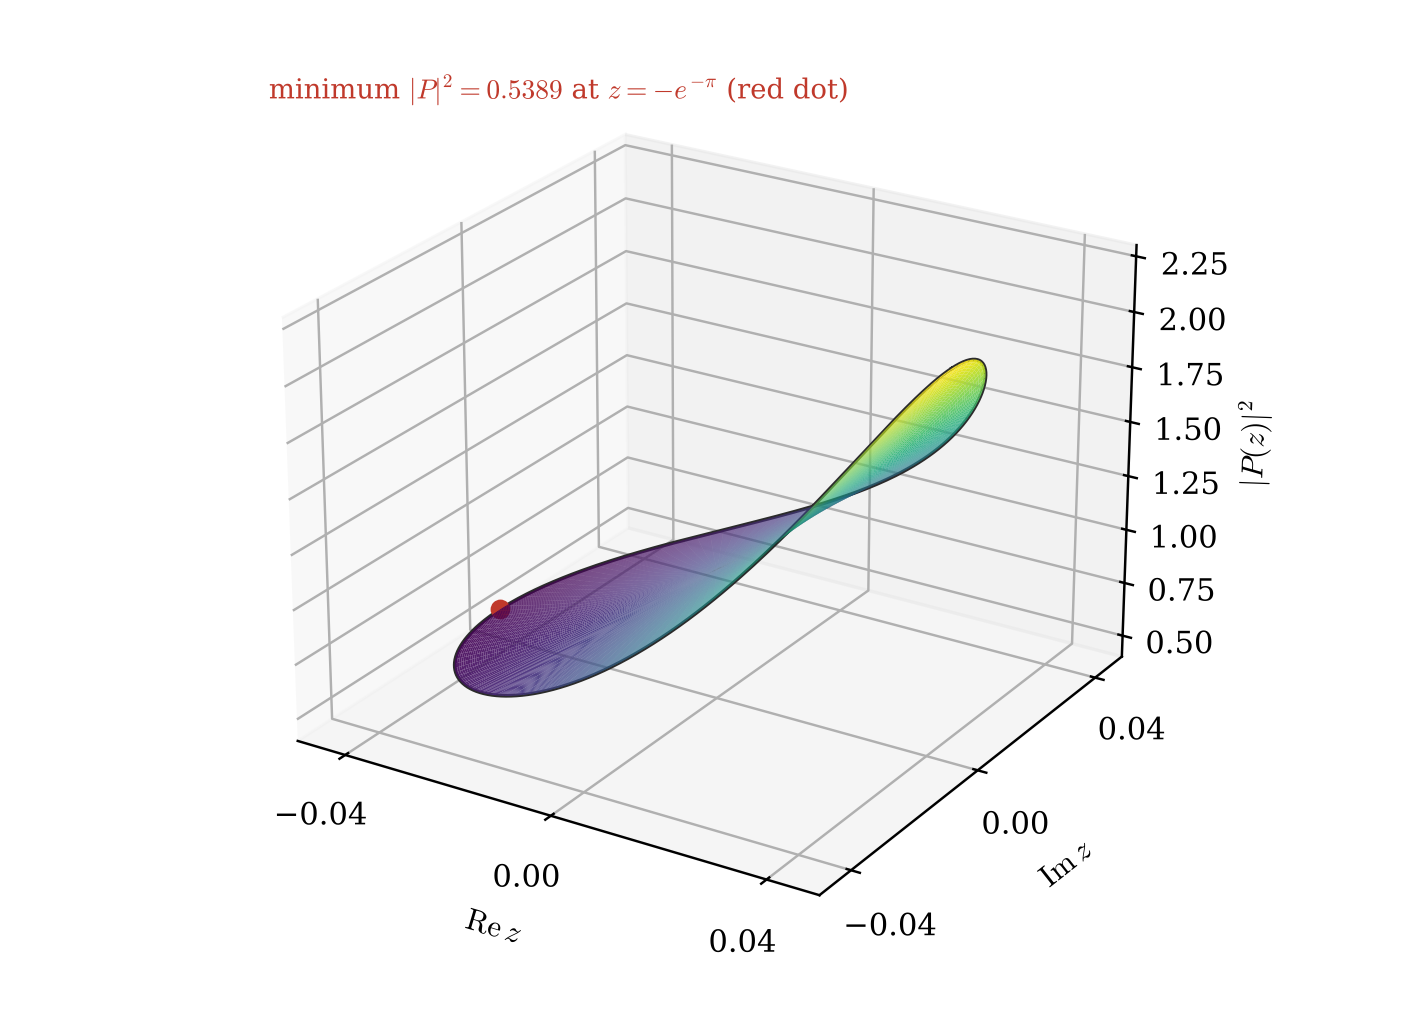
\includegraphics[width=0.78\textwidth]{fig_pdisc.png}
\caption{The surface $|P(z)|^2$ over the disc $|z|\le e^{-\pi}$, where $z=e^{-\pi x+i\theta}$ with $x\ge1$. The rim is the image of $x=1$; the lowest point is $z=-e^{-\pi}$, which corresponds to $x=1$ and $\ell=m$ odd.}\label{fig:pdisc}
\end{figure}

\begin{remark}\label{rem:physics}
The function $1/(\eta(\tau)^8\eta(2\tau)^8)$, whose coefficients are $d_1$, is the generating function of the electric half-BPS degeneracies of the model \cite{Sen08}. Theorem~\ref{thm:model} therefore says that, to leading order, the single-centred index of a quarter-BPS black hole is the extreme Bessel term times the squared modulus of the half-BPS generating function, evaluated at the point $z=e^{-\pi\sqrt D/Q^2+i\pi Q\cdot P/Q^2}$. The positivity of $|P|^2$ is automatic; what has to be proved is that the corrections cannot overturn it, and Proposition~\ref{prop:pmin} gives the room.
\end{remark}

\section{Facts on Bessel functions}\label{sec:bessel}

All Bessel functions below have real order $\nu\ge\frac12$ and positive argument. We use
\begin{equation}\label{eq:gdef}
g(y)=\sqrt{2\pi y}\,e^{-y}I_{15/2}(y),\qquad \phi(y)=\frac{y\,g'(y)}{g(y)}.
\end{equation}

\begin{lemma}\label{lem:besselbasic}
\begin{enumerate}
\item[(i)] $I_\nu(z)/z^\nu$ is increasing; hence $I_\nu(z/\gamma)\le\gamma^{-\nu}I_\nu(z)$ for $\gamma\ge1$.
\item[(ii)] $z\,I_\nu'(z)/I_\nu(z)$ is increasing in $z$. Consequently, for $0<c\le1$ the function $y\mapsto I_\nu(cy)/I_\nu(y)$ is nonincreasing.
\item[(iii)] For $\nu'\ge\nu$, $z\,I_{\nu'}'(z)/I_{\nu'}(z)\le(\nu'-\nu)+z\,I_\nu'(z)/I_\nu(z)$.
\item[(iv)] For fixed $z>0$, $I_\nu(z)$ is nonincreasing in $\nu\ge0$.
\item[(v)] $I_\nu(z)\le\dfrac{(z/2)^\nu}{\Gamma(\nu+1)}e^{z^2/4}$.
\end{enumerate}
\end{lemma}

\begin{proof}
(i) $I_\nu(z)/z^\nu=2^{-\nu}\sum_k(z^2/4)^k/(k!\,\Gamma(\nu+k+1))$ has positive coefficients. (v) follows from the same series and $\Gamma(\nu+k+1)\ge\Gamma(\nu+1)$. For (ii) and (iii) we use the Weierstrass product $I_\nu(z)=\frac{(z/2)^\nu}{\Gamma(\nu+1)}\prod_{k\ge1}\big(1+z^2/j_{\nu,k}^2\big)$, where $0<j_{\nu,1}<j_{\nu,2}<\dots$ are the positive zeros of $J_\nu$ \cite[\S15.41]{Wat44}. It gives
\[
\frac{zI_\nu'(z)}{I_\nu(z)}=\nu+\sum_{k\ge1}\frac{2z^2}{j_{\nu,k}^2+z^2},
\]
each summand increasing in $z$, which is the first part of (ii). For the second, $\frac{d}{dy}\log\frac{I_\nu(cy)}{I_\nu(y)}=\frac1y\Big(\frac{cyI_\nu'(cy)}{I_\nu(cy)}-\frac{yI_\nu'(y)}{I_\nu(y)}\Big)\le0$. For (iii), the zeros $j_{\nu,k}$ increase with $\nu$ \cite[\S15.6]{Wat44}, so each summand for $\nu'$ is at most the one for $\nu$. (iv) is a theorem of Cochran \cite{Coc67}.
\end{proof}

\begin{lemma}\label{lem:gfacts}
\begin{enumerate}
\item[(i)] $0<g(y)<1$ for all $y>0$, and $g(y)\to1$ as $y\to\infty$.
\item[(ii)] $\phi$ is positive and decreasing on $[3,\infty)$; in particular $g$ is increasing on $[3,\infty)$, and for $0<c\le1$ the ratio $g(cy)/g(y)$ is nondecreasing on $\{y:\ cy\ge3\}$.
\item[(iii)] $y\,\phi(y)\le29$ for $y\ge30$; hence $g'(y)\le29/y^2$ there.
\item[(iv)] $\sqrt{2\pi y}\,e^{-y}I_\nu(y)\le1$ for every $\nu\ge\frac{15}2$ and $y>0$.
\end{enumerate}
\end{lemma}

\begin{proof}
For half-integral order there is the closed form \cite[\S3.71]{Wat44}
\begin{equation}\label{eq:halfint}
g(y)=p\Big(-\frac1{2y}\Big)+e^{-2y}p\Big(\frac1{2y}\Big),\qquad p(w)=\sum_{k=0}^7\frac{(7+k)!}{k!\,(7-k)!}w^k ,
\end{equation}
which gives $g(y)\to1$. Write $r=I_{17/2}/I_{15/2}$; the recurrences give $\phi=8-y+yr$ and $\phi'=y-1-15r-yr^2$ (we use $I_\nu'=I_{\nu+1}+\frac\nu yI_\nu$ and $r'=1-\frac{16}yr-r^2$). On $[3,60]$ we enclose $\phi'$ on a cover of the interval by boxes, in ball arithmetic, by the mean value form $\phi'(c)+[-\frac h2,\frac h2]\,\phi''(\text{box})$; every enclosure is negative. On $[60,\infty)$ we use \eqref{eq:halfint}: with $w=1/2y$, the main part $w\,p'(-w)/p(-w)$ of $\phi$ has positive derivative in $w$ on $(0,\frac1{120}]$ (checked on $600$ subintervals), and the remaining part is $O(y^2e^{-2y})$ together with its derivative, which is far smaller. This proves that $\phi$ is decreasing on $[3,\infty)$, and $\phi(60)>0$ together with $\phi\to0^+$ gives positivity. Since $g$ increases on $[3,\infty)$ to the limit $1$, $g<1$ there; on $(0,3]$, (v) of Lemma~\ref{lem:besselbasic} gives $g(y)\le\sqrt{6\pi}\,(3/2)^{15/2}e^{9/4-3}/\Gamma(17/2)<0.01$. The monotonicity of $g(cy)/g(y)$ is (ii) of Lemma~\ref{lem:besselbasic} with $\phi$ in place of $zI'/I$. (iii) on $[30,60]$ is checked on a grid of step $0.05$ using that $\phi$ is decreasing, and on $[60,\infty)$ from the closed form, where $y\phi(y)\le\frac12p'(-w)/p(-w)+O(y^3e^{-2y})<28$. Finally (iv) follows from (i) and Lemma~\ref{lem:besselbasic}(iv).
\end{proof}

The following monotonicity in $x$ is what makes every bound of Section~\ref{sec:errors}, proved at the smallest admissible $x$, valid for all larger $x$.

\begin{lemma}\label{lem:xmono}
Let $x=\sqrt D/m$ and let $\mathcal E(D,m)$ be as in \eqref{eq:ext}. For a constant $0<c\le\pi\sqrt{t_0}$, each of the following ratios is a nonincreasing function of $x>0$:
\[
\frac{D^{-15/4}I_{15/2}(cx)}{\mathcal E(D,m)},\qquad\frac{D^{-4}I_8(cx)}{\mathcal E(D,m)},\qquad\frac{D^{-17/4}I_{17/2}(cx)}{\mathcal E(D,m)}.
\]
\end{lemma}

\begin{proof}
Up to constants, $\mathcal E=D^{-15/4}I_{15/2}(c_0x)$ with $c_0=\pi\sqrt{t_0}\ge c$, and $D=m^2x^2$. The first ratio is $I_{15/2}(cx)/I_{15/2}(c_0x)$, nonincreasing by Lemma~\ref{lem:besselbasic}(ii). The logarithmic derivative in $x$ of the second is
\[
\frac1x\Big(-\frac12+\frac{cxI_8'(cx)}{I_8(cx)}-\frac{c_0xI_{15/2}'(c_0x)}{I_{15/2}(c_0x)}\Big)\le\frac1x\Big(-\frac12+\frac12+\frac{cxI_{15/2}'(cx)}{I_{15/2}(cx)}-\frac{c_0xI_{15/2}'(c_0x)}{I_{15/2}(c_0x)}\Big)\le0
\]
by Lemma~\ref{lem:besselbasic}(iii) and (ii). The third is the same with $-1$ and $+1$.
\end{proof}

\begin{remark}
In Lemma~\ref{lem:xmono} the extra power $D^{-1/4}$ of the shadow terms exactly compensates the higher order of the Bessel function. This is the level-two counterpart of the fact, used in \cite{BMa13,Ros24}, that the shadow terms of a mixed mock form grow at most like its principal-part terms.
\end{remark}

\begin{lemma}\label{lem:d1bound}
For $n\ge-1$, $0<d_1(n)\le e^{2\pi\sqrt{2(n+1)}}$. More generally $d_1(n)\le P(q)\,q^{-(n+1)}$ for every $0<q<1$.
\end{lemma}

\begin{proof}
Positivity is clear from the product. The second bound holds since $P(q)=\sum d_1(a)q^{a+1}$ has nonnegative coefficients. With $q=e^{-\tau}$, comparison of the sum with an integral gives $\sum_{k\ge1}-\log(1-e^{-k\tau})\le\int_0^\infty-\log(1-e^{-u\tau})\,du=\pi^2/6\tau$, so $\log P(e^{-\tau})\le8\cdot\frac{\pi^2}{6\tau}+8\cdot\frac{\pi^2}{12\tau}=\frac{2\pi^2}\tau$. Taking $\tau=\pi\sqrt{2/(n+1)}$ gives the first bound.
\end{proof}

\section{Bounds for the remaining terms}\label{sec:errors}

Throughout this section $(m,n,\ell)$ is a reduced charge, $x=\sqrt D/m\ge x_0\ge1$, and all bounds are uniform in $\ell$ and in $x\ge x_0$. We write $B_\gamma(t;x)=(t/t_0)^{15/4}I_{15/2}(\pi x\sqrt t/\gamma)/I_{15/2}(\pi x\sqrt{t_0})$ and $u=e^{-\pi}$. By Lemma~\ref{lem:besselbasic}(i),(ii), $B_\gamma(t;x)$ is increasing in $t$ and nonincreasing in $x$, and $B_\gamma\le\gamma^{-15/2}B_1$.

\subsection{Decomposition}
By Theorem~\ref{thm:rad}, $d^*(m,n,\ell)=\frac12(-1)^\ell\sqrt i(\mathcal M+\mathcal K_2+\mathcal K_3)$, and Theorem~\ref{thm:model} splits this as
\begin{equation}\label{eq:decomp}
\frac{d^*(m,n,\ell)}{\mathcal E(D,m)}=|P(z)|^2-\mathcal X_{\rm miss}+\mathcal X_{\rm main}+\mathcal X_{rs}+\mathcal X_{T}+\mathcal X_{\gamma\ge2}+\mathcal X_{K_2}+\mathcal X_{K_3},
\end{equation}
where
\begin{itemize}
\item $\mathcal X_{\rm miss}=\sum d_1(a)d_1(b)e^{-\pi xS}\cos((a-b)\theta)$ over the pairs $a,b\ge-1$ not in $\mathcal L_m$;
\item $\mathcal X_{\rm main}=\sum_{(a,b)\in\mathcal L_m}d_1(a)d_1(b)\big(\rho_{a,b}(x)-e^{-\pi xS}\big)\cos((a-b)\theta)$;
\item $\mathcal X_{rs}$ is the contribution of the walls with $rs\ge2$ to the frame $S$ term with $\gamma=1$, divided by $\mathcal E$;
\item $\mathcal X_T$ is the frame $T$ term with $\gamma=1$, divided by $\mathcal E$;
\item $\mathcal X_{\gamma\ge2}$ collects the terms of $\mathcal M$ with $\gamma\ge2$, and $\mathcal X_{K_j}$ the term $\frac12(-1)^\ell\sqrt i\,\mathcal K_j$, divided by $\mathcal E$.
\end{itemize}
We bound each piece in absolute value.

\subsection{Parametrising the walls}
\begin{lemma}\label{lem:wallparam}
The map sending a polar term $(\tilde\nu,\tilde\ell)$ with $0\le\tilde\ell<2m$ and a wall $G\in\mathcal W(m,\tilde\nu,\tilde\ell)$ to $(r,s,m_G,n_G)$ is injective. Given $(r,s,a,b)$ in its image, $\delta$ is the unique solution of
\begin{equation}\label{eq:deltaeq}
\sqrt{\delta^2+\frac a{mr^2}}+\sqrt{\delta^2+\frac b{ms^2}}=\frac1{rs},
\end{equation}
so $t=4m^2\delta^2$ is a function $t(r,s,a,b)$, and $\ell_G\le m-a-b$.
\end{lemma}

\begin{proof}
By Lemma~\ref{lem:walls}(ii), $U=\sqrt{\delta^2+a/mr^2}$ and $W=\sqrt{\delta^2+b/ms^2}$, and $U+W=1/rs$; the left side of \eqref{eq:deltaeq} is increasing in $\delta^2$, which gives uniqueness, and $\ell_G=2mrs(UW+\delta^2)$ is then determined. The form $\phi\circ G$ has coefficients $(n_G,-\ell_G,m_G)$ up to the order of the variables, so it is determined; given $(r,s)$, the matrices $G$ are $\begin{psmallmatrix}p_0+kr&q_0+ks\\r&s\end{psmallmatrix}$, $k\in\ZZ$; for a fixed form $\phi\circ G$ the choice of $k$ shifts $\omega_0=\tilde\ell/2m$ by the integer $k$, that is, $\tilde\ell$ by $2mk$; the condition $0\le\tilde\ell<2m$ fixes $k$, and then $\phi=(\phi\circ G)\circ G^{-1}$ is determined. Finally $\ell_G=m-a-b-E_G\le m-a-b$ by Lemma~\ref{lem:walls}(iii).
\end{proof}

\subsection{The leading family}
\begin{lemma}\label{lem:mainerr}
Let $(a,b)\in\mathcal L_m$ with $S\ge1$, and put $c_0=\frac k{m+2}(t/t_0)^{7/2}$ and $\hat g_0=g(\pi x_0\sqrt t)/g(\pi x_0\sqrt{t_0})$. Then
\[
\sup_{x\ge x_0}\big|\rho_{a,b}(x)-e^{-\pi xS}\big|\le\max_{C\in\{c_0,\,c_0\hat g_0\}}\ \sup_{x\ge x_0}\big|Ce^{-\pi\Delta_sx}-e^{-\pi Sx}\big| .
\]
\end{lemma}

\begin{proof}
From $I_{15/2}(y)=g(y)e^y/\sqrt{2\pi y}$ one gets $\rho_{a,b}(x)=c_0\,\hat g(x)\,e^{-\pi\Delta_sx}$ with $\hat g(x)=g(\pi x\sqrt t)/g(\pi x\sqrt{t_0})$. Since $t\ge1$, $\pi x\sqrt t\ge3$, and Lemma~\ref{lem:gfacts}(ii) shows $\hat g_0\le\hat g(x)\le1$. The expression is affine in $\hat g$, so its modulus is at most the larger of the values at the two ends.
\end{proof}

The supremum of $|Ce^{-\alpha x}-e^{-\beta x}|$ on $[x_0,\infty)$ is attained at $x_0$ or at the unique critical point $x_*=\log(\beta/C\alpha)/(\beta-\alpha)$ when $x_*>x_0$, and is computed exactly. Summing,
\begin{equation}\label{eq:Xmain}
|\mathcal X_{\rm main}|\le\sum_{(a,b)\in\mathcal L_m,\ S\ge1}d_1(a)d_1(b)\max_{C}\sup_{x\ge x_0}\big|Ce^{-\pi\Delta_sx}-e^{-\pi Sx}\big|=:\epsilon_{\rm main}(m,x_0),
\end{equation}
\begin{equation}\label{eq:Xmiss}
|\mathcal X_{\rm miss}|\le\sum_{(a,b)\notin\mathcal L_m}d_1(a)d_1(b)u^{x_0S}=:\epsilon_{\rm miss}(m,x_0).
\end{equation}
The pairs not in $\mathcal L_m$ have $S\ge m/2+2$ (if $t\le0$ then $(m+2-S)^2\le4ab\le(S-2)^2$) or $|a-b|\ge m$ (so $S\ge m$) or $k\le0$; we sum them exactly for $S\le4m+10$, and for larger $S$ use $\sum_{a+b=S-2}d_1(a)d_1(b)\le P(q_1)^2q_1^{-S}$ with $q_1=u^{x_0/2}$, by Lemma~\ref{lem:d1bound}.

For large $m$ a coarser bound is convenient.

\begin{lemma}\label{lem:mainS}
Let $m\ge3$, $x_0=1$, $1\le S\le m+1$, and let $\eta_\pm$ be as in Lemma~\ref{lem:deltas}. Assume $S-\eta_-\ge1/\pi$. Then every $(a,b)\in\mathcal L_m$ with $a+b+2=S$ satisfies
\[
\sup_{x\ge1}\big|\rho_{a,b}(x)-e^{-\pi xS}\big|\le u^S\,\varphi(S,m),\qquad \varphi(S,m)=\epsilon_1+e^{\pi\eta_-}-1+\min(1,\pi\eta_+),
\]
where $\epsilon_1=\min\big(1,\ \frac{8S}m+\frac{29\pi(S+\eta_+)}{y_t^2g(y_t)}\big)$ with $y_t=\pi\sqrt{t_0-2mS}$ if $y_t\ge30$, and $\epsilon_1=1$ otherwise.
\end{lemma}

\begin{proof}
Write $\rho=c_0\hat g\,e^{-\pi x\Delta_s}=c\,e^{\pi xy}e^{-\pi xS}$ with $c=c_0\hat g\le1$ and $y=S-\Delta_s\in[-\eta_+,\eta_-]$. Then $|ce^{\pi xy}-1|\le c|e^{\pi xy}-1|+(1-c)\le(e^{\pi x\eta_-}-1)+\min(1,\pi x\eta_+)+(1-c)$. First, $1-c\le(1-\frac k{m+2})+(1-(t/t_0)^{7/2})+(1-\hat g)$; here $1-\frac k{m+2}=\frac S{m+2}$, $1-(t/t_0)^{7/2}\le\frac72\cdot\frac{2mS}{t_0}\le\frac{7S}m$ by Lemma~\ref{lem:deltas}(i), and, with $z=\pi x\sqrt t\ge y_t$ and $z_0=\pi x\sqrt{t_0}$, Lemma~\ref{lem:gfacts}(ii),(iii) give
\[
1-\hat g\le\frac{g(z_0)-g(z)}{g(z)}\le\frac{29(z_0-z)}{z^2g(z)}\le\frac{29\pi x(S+\eta_+)}{\pi^2x^2t\,g(y_t)}\le\frac{29\pi(S+\eta_+)}{y_t^2g(y_t)}
\]
when $y_t\ge30$; trivially $1-c\le1$. Multiply by $e^{-\pi xS}$. The function $e^{-\pi xS}(e^{\pi x\eta_-}-1)=e^{-\pi x(S-\eta_-)}-e^{-\pi xS}$ is nonincreasing on $[1,\infty)$ as soon as $S/(S-\eta_-)\le e^{\pi\eta_-}$, which follows from $e^{\pi\eta_-}\ge1+\pi\eta_-$ and $S-\eta_-\ge1/\pi$; the function $xe^{-\pi xS}$ is decreasing for $x\ge1/\pi S$; and the bound for $1-c$ is nonincreasing in $x$. So the supremum is at most the value at $x=1$.
\end{proof}

\subsection{The other walls at \texorpdfstring{$\gamma=1$}{gamma=1}}
Dividing \eqref{eq:gamma1S} restricted to $a_S^{\rm rest}$, and the frame $T$ term, by $\mathcal E$, and using $|W_{1,\delta}|=(2m)^{-1/2}$, Lemma~\ref{lem:wallparam} and the monotonicity of $B_1$,
\begin{align}
|\mathcal X_{rs}|&\le\frac1{m+2}\sum_{\substack{r,s\le2m,\ rs\ge2\\ a,b\ge-1}}(m-a-b)\,d_1(a)d_1(b)\,B_1\big(t(r,s,a,b);x_0\big)=:\epsilon_{rs},\label{eq:Xrs}\\
|\mathcal X_T|&\le\frac{16}{m+2}\sum_{\substack{r,s\le2m\\ r\ \text{or}\ s\ \text{even}}}\ \sum_{a,b\in\frac12\ZZ}(m-a-b)\,w(r,s,a,b)\,B_1\big(t(r,s,a,b);x_0\big)=:\epsilon_T,\label{eq:XT}
\end{align}
where $w=d_1(a)d_1(2b)$ if $r$ is even and $w=d_1(2a)d_1(b)$ if $s$ is even. The ranges are finite by Lemma~\ref{lem:walls}(v): $a\le m/s^2$, $b\le m/r^2$. Only quadruples for which \eqref{eq:deltaeq} has a solution occur; in the certificate an upper bound for $\delta^2$ is found by bisection and then certified in ball arithmetic, and a quadruple is discarded only when the left side of \eqref{eq:deltaeq} exceeds $1/rs$ already at the least admissible $\delta^2$, again certified.

For $m\ge101$ we use instead the following bound.

\begin{lemma}\label{lem:rsbig}
For $m\ge101$, with $c=\frac{m-1}{4(m+2)}$, $q=e^{-\pi c}$, $A_1=\frac m2-3-\frac2m$ and $g_0=g(\pi\sqrt{t_0})$,
\[
|\mathcal X_{rs}|+|\mathcal X_T|\le\frac{(2m+1)^2\big(P(q)^2+64\sqrt q\,P(q)P(\sqrt q)\big)e^{-\pi A_1/2}}{g_0}.
\]
\end{lemma}

\begin{proof}
For a wall with $rs\ge2$, Lemma~\ref{lem:walls}(vi) gives $\sqrt t\le\frac m2+5$, and $\sqrt{t_0}\ge m+2-\frac2m$, so $\Delta_s=\sqrt{t_0}-\sqrt t\ge A_1$. Also $\Delta_s\ge S(2m-S)/(2(m+2))$ with $S=a+b+2\le m+1$ (by Lemma~\ref{lem:walls}(ii), $a+b\le m(r^2U^2+s^2W^2)$, and on the segment $U+W=1/rs$ this convex function is at most $m\max(r^{-2},s^{-2})\le m$; $a+b=m$ is excluded since $\ell_G\le m-a-b$ must be positive), hence $\Delta_s\ge2cS$. So $e^{-\pi x\Delta_s}\le e^{-\pi A_1/2}q^S$. As in Lemma~\ref{lem:mainerr}, $B_1(t;x)\le(t/t_0)^{7/2}e^{-\pi x\Delta_s}g(\pi x\sqrt t)/g(\pi x\sqrt{t_0})\le e^{-\pi x\Delta_s}/g_0$. With $m-a-b\le m+2$, the sum over $(a,b)$ of $d_1(a)d_1(b)q^S$ is at most $P(q)^2$, the sum of $d_1(a)d_1(2b)q^{a+b+2}$ over $a\in\ZZ$, $b\in\frac12\ZZ$ is at most $\sqrt q\,P(q)P(\sqrt q)$, and there are at most $(2m)^2$ pairs $(r,s)$. The factor $64$ accounts for the factor $16$, the two parity types and a factor $2$ of room.
\end{proof}

\subsection{The terms with \texorpdfstring{$\gamma\ge2$}{gamma>=2}}
Let $N_F(\gamma)$ be the number of $\delta$ with $(\gamma,\delta)\in\mathcal C_\gamma$ and frame $F$; then $N_I+N_T+N_S\le2\gamma$. Each term of $\mathcal M$ with $\gamma\ge2$, divided by $\mathcal E$, is at most $\frac{16}{m+2}|a_F|\cdot\sqrt{2m}\,|W|\cdot\gamma^{-1}B_\gamma(t;x)$, and $\sqrt{2m}|W|\le\sqrt{2\gcd(m,\gamma)}$ by Lemma~\ref{lem:weilbound}. Bounding $|a_S|$ and $|a_I|$ by the sums of the absolute values of their walls,
\begin{equation}\label{eq:Xg2}
\begin{split}
|\mathcal X_{\gamma\ge2}|&\le\sum_{\gamma=2}^{G}\frac{\sqrt{2\gcd(m,\gamma)}}{\gamma}\big(N_S(\gamma)\Sigma_S(\gamma)+(N_I+N_T)(\gamma)\,\Sigma_T(\gamma)\big)\\
&\quad+\frac{2\sqrt2\,(\Sigma_S(1)+\Sigma_T(1))}{6G^6}=:\epsilon_{\gamma\ge2},
\end{split}
\end{equation}
where $\Sigma_S(\gamma)$ and $\Sigma_T(\gamma)$ are the sums \eqref{eq:Xrs} (including the leading family) and \eqref{eq:XT} with $B_1$ replaced by $B_\gamma$. The tail uses $B_\gamma\le\gamma^{-15/2}B_1$, $N\le2\gamma$, $\gcd(m,\gamma)\le\gamma$ and $\sum_{\gamma>G}\gamma^{-7}\le G^{-6}/6$. We take $G=12$.

\begin{lemma}\label{lem:g2big}
For $m\ge101$, with $q,g_0$ as in Lemma~\ref{lem:rsbig},
\[
|\mathcal X_{\gamma\ge2}|\le2^9\big(\zeta(7)-1\big)\sqrt2\,e^{-\pi\sqrt{t_0}/2}\,\frac{(2m+1)^2\big(P(q)^2+64\sqrt q\,P(q)P(\sqrt q)\big)}{g_0}.
\]
\end{lemma}

\begin{proof}
By Lemma~\ref{lem:besselbasic}(i), $I(z/\gamma)\le(2/\gamma)^{15/2}I(z/2)$ for $\gamma\ge2$. By Lemma~\ref{lem:gfacts}(i), $I(z/2)\le e^{z/2}/\sqrt{\pi z}$, and $I(z_0)=g(z_0)e^{z_0}/\sqrt{2\pi z_0}$, so $(t/t_0)^{15/4}I(z/2)/I(z_0)\le\sqrt2e^{-z_0/2}e^{-(z_0-z)/2}/g_0\le\sqrt2e^{-\pi\sqrt{t_0}/2}q^S/g_0$, using $(t/t_0)^{15/4}(t_0/t)^{1/4}\le1$ and $\Delta_s\ge2cS$ as before. Finally $\sum_{\gamma\ge2}2\gamma\cdot\sqrt{2\gamma}\,\gamma^{-1}(2/\gamma)^{15/2}=2^9\sum_{\gamma\ge2}\gamma^{-7}$.
\end{proof}

\subsection{The shadow terms}
By \eqref{eq:fsum} and Lemma~\ref{lem:weilbound}, with $\psi_1=(2m)^{-1/2}$ and $\psi_\gamma=\sqrt{\gcd(m,\gamma)/m}$, and $D_0=m^2x_0^2$,
\begin{align}
|\mathcal X_{K_2}|&\le\sum_{\gamma\ge1}\sum_F\frac{N_F(\gamma)}2\cdot\frac{\sqrt{2m}\,|c_F|\,\psi_\gamma}{\sqrt\gamma}\Big(\frac{4m\mu_F}{D_0}\Big)^4\frac{I_{15/2}\big(2\pi x_0\sqrt{\mu_Fm}/\gamma\big)}{\mathcal E(D_0,m)},\label{eq:XK2}\\
|\mathcal X_{K_3}|&\le\sum_{\gamma\ge1}\sum_F\frac{N_F(\gamma)}2\cdot\frac{|c_F|\,\psi_\gamma}{2\pi\gamma^2}\Big(\frac{4m\mu_F}{D_0}\Big)^{\frac{17}4}\cdot2\sqrt{\frac{\mu_F}m}\cdot\frac{4\pi^2m^2\gamma^2}3\cdot\frac{I_{15/2}\big(2\pi x_0\sqrt{\mu_Fm}/\gamma\big)}{\mathcal E(D_0,m)}.\label{eq:XK3}
\end{align}
Indeed, the arguments of $I_8$ and $I_{17/2}$ are $c\,x$ with $c\le2\pi\sqrt m\le\pi\sqrt{t_0}$, so by Lemma~\ref{lem:xmono} each term divided by $\mathcal E$ is largest at $x=x_0$; there $I_8,I_{17/2}\le I_{15/2}$ by Lemma~\ref{lem:besselbasic}(iv), the factor $(1-mu^2/\mu_F)^{17/4}$ is at most $1$, $I_{17/2}$ is increasing in its argument, and the interval of integration has length $2\sqrt{\mu_F/m}$. The certificate sums $\gamma\le G=12$ exactly and bounds the rest using $I_{15/2}(z/\gamma)\le\gamma^{-15/2}I_{15/2}(z)$, $N\le2\gamma$ and $\psi_\gamma\le1$, with $\sum_{\gamma>G}\gamma^{-7}\le G^{-6}/6$ for \eqref{eq:XK2} and $\sum_{\gamma>G}\gamma^{-13/2}\le\frac2{11}G^{-11/2}$ for \eqref{eq:XK3}.

\begin{lemma}\label{lem:mockbig}
For $m\ge101$, with $z_0=\pi\sqrt{t_0}$, $z_1=2\pi\sqrt m$ and $J=\sqrt{z_0/z_1}\,e^{z_1-z_0}/g(z_0)$,
\[
|\mathcal X_{K_2}|\le\frac{\sqrt{2m}\,\frac{17}{16}e^{2\pi\sqrt{2m+2}}(4/m)^4\zeta(7)J}{\frac{\pi}{\sqrt{2m}}\frac{m+2}{16}},\qquad |\mathcal X_{K_3}|\le\frac{\frac{17}{16}e^{2\pi\sqrt{2m+2}}\frac{1}{2\pi}(4/m)^{17/4}\frac2{\sqrt m}\frac{4\pi^2m^2}3\zeta(\frac{13}2)J}{\frac{\pi}{\sqrt{2m}}\frac{m+2}{16}}.
\]
\end{lemma}

\begin{proof}
Take $x_0=1$ in \eqref{eq:XK2}, \eqref{eq:XK3}. Use $|c_F|\le\hat f(m)\le e^{2\pi\sqrt{2m+2}}$ (Lemma~\ref{lem:d1bound}), $\mu_F\le1$, $\psi_\gamma\le1$, $N\le2\gamma$, $I_{15/2}(z_1/\gamma)\le\gamma^{-15/2}I_{15/2}(z_1)$, and $\mathcal E(m^2,m)\ge\frac\pi{\sqrt{2m}}\frac{m+2}{16}I_{15/2}(z_0)$. Finally $I_{15/2}(z_1)/I_{15/2}(z_0)\le J$ by Lemma~\ref{lem:gfacts}(i).
\end{proof}

\section{Proof of Theorem~\ref{thm:all}}\label{sec:proofall}

Let $\epsilon(m,x_0)=\epsilon_{\rm main}+\epsilon_{\rm miss}+\epsilon_{rs}+\epsilon_T+\epsilon_{\gamma\ge2}+\epsilon_{K_2}+\epsilon_{K_3}$ be the sum of the bounds of Section~\ref{sec:errors}, where $\epsilon_{K_j}$ denote the right sides of \eqref{eq:XK2} and \eqref{eq:XK3} with the tails included.

\begin{theorem}\label{thm:cert}
Put $x_0(m)=\sqrt{500}/m$ for $3\le m\le7$ and $x_0(m)=1$ for $8\le m\le100$. Then
\[
\epsilon\big(m,x_0(m)\big)\le0.347\qquad(3\le m\le100),
\]
with the largest value at $m=8$; for $3\le m\le7$ one has $\epsilon\le0.0025$.
\end{theorem}

\begin{proof}
Every term of $\epsilon(m,x_0)$ is a finite sum of explicit quantities, which we evaluate in ball arithmetic with $96$ bits \cite{Joh17}. Bessel functions are evaluated by Arb's certified routines, the suprema in \eqref{eq:Xmain} by the exact critical points, and the solutions of \eqref{eq:deltaeq} are enclosed as described after \eqref{eq:XT}. The values are listed in Appendix~\ref{app:margins} and plotted in Figure~\ref{fig:certificate}; the computation takes about twelve minutes.
\end{proof}

\begin{theorem}\label{thm:analytic}
For every $m\ge101$, $\epsilon(m,1)\le0.3382$.
\end{theorem}

\begin{proof}
\emph{Leading family and missing pairs.} Group the pairs by $S$. For $1\le S\le m+1$, Lemma~\ref{lem:deltas} gives $S-\eta_-=S(2m-S)/(2m+4)\ge(2m-1)/(2m+4)>1/\pi$, so Lemma~\ref{lem:mainS} applies, and the pairs with $a+b+2=S$ contribute at most $p_2(S)u^S\varphi(S,m)$, where $p_2(S)=\sum_{a+b=S-2}d_1(a)d_1(b)$. Missing pairs have $S\ge m/2+2$ and contribute at most $p_2(S)u^S$. For $S>300$ we use, for the pairs in $\mathcal L_m$, $|\rho_{a,b}-e^{-\pi xS}|\le e^{-\pi\Delta_s}+e^{-\pi S}\le2e^{-\pi S(m-1)/(2m+4)}\le2e^{-0.485\pi S}$ (Lemma~\ref{lem:deltas}(iv)), and $p_2(S)\le P(q)^2q^{-S}$ with $q=e^{-0.4\pi}$, so these terms add up to at most $2P(q)^2\varrho^{301}/(1-\varrho)$ with $\varrho=e^{-0.485\pi}/q$. Evaluated in ball arithmetic, the total is at most $0.33815$ for every $101\le m\le300$, the largest value being at $m=101$.

For $m>300$ we compare with $m=300$. The bound $\eta_-$ decreases in $m$; for $S\le3$ one checks $\eta_+=0$ (for $S=3$ this is $\sqrt{1+4/m}+\sqrt{1-2/m}\ge2$, true for $m\ge3$), and for $S\ge4$ the function $\sqrt{m(m+4)}-\sqrt{m(m+4-2S)}=2S/\big(\sqrt{1+4/m}+\sqrt{1+(4-2S)/m}\big)$ decreases in $m$; $y_t=\pi\sqrt{m(m+4-2S)}$ increases, and $8S/m$ decreases. Hence $\varphi(S,m)\le\varphi(S,300)$ whenever $2S\le304$. For $152<S\le300$ the term $\varphi(S,300)$ has $\epsilon_1=1$ and $\min(1,\pi\eta_+)=1$, so again $\varphi(S,m)\le\varphi(S,300)$. The missing pairs for $m>300$ have $S\ge m/2+2>152$, and their terms $p_2(S)u^S$ with $S\le300$ are counted at $m=300$; those with $S>300$ are in the tail. So the bound at $m=300$, which is $0.1090$, holds for all $m>300$.

\emph{The other pieces.} By Lemmas~\ref{lem:rsbig}, \ref{lem:g2big} and~\ref{lem:mockbig}, with $q=q(101)$ (since $c$ increases with $m$, the bound with $q(101)$ holds for all $m\ge101$),
\[
|\mathcal X_{rs}|+|\mathcal X_T|\le3.02\cdot10^{-8},\quad|\mathcal X_{\gamma\ge2}|\le3\cdot10^{-45},\quad|\mathcal X_{K_2}|\le6\cdot10^{-79},\quad|\mathcal X_{K_3}|\le7\cdot10^{-77}
\]
at $m=101$. Each bound decreases in $m$: in Lemma~\ref{lem:rsbig} the factor $(2m+1)^2e^{-\pi m/4}$ decreases for $m\ge101$ and $g_0$ increases; in Lemma~\ref{lem:g2big} the factor $e^{-\pi\sqrt{t_0}/2}$ dominates; in Lemma~\ref{lem:mockbig} the exponent $2\pi\sqrt{2m+2}+z_1-z_0\le2\pi\sqrt{2m+2}+2\pi\sqrt m-\pi m$ decreases.
\end{proof}

\begin{figure}[t]
\centering
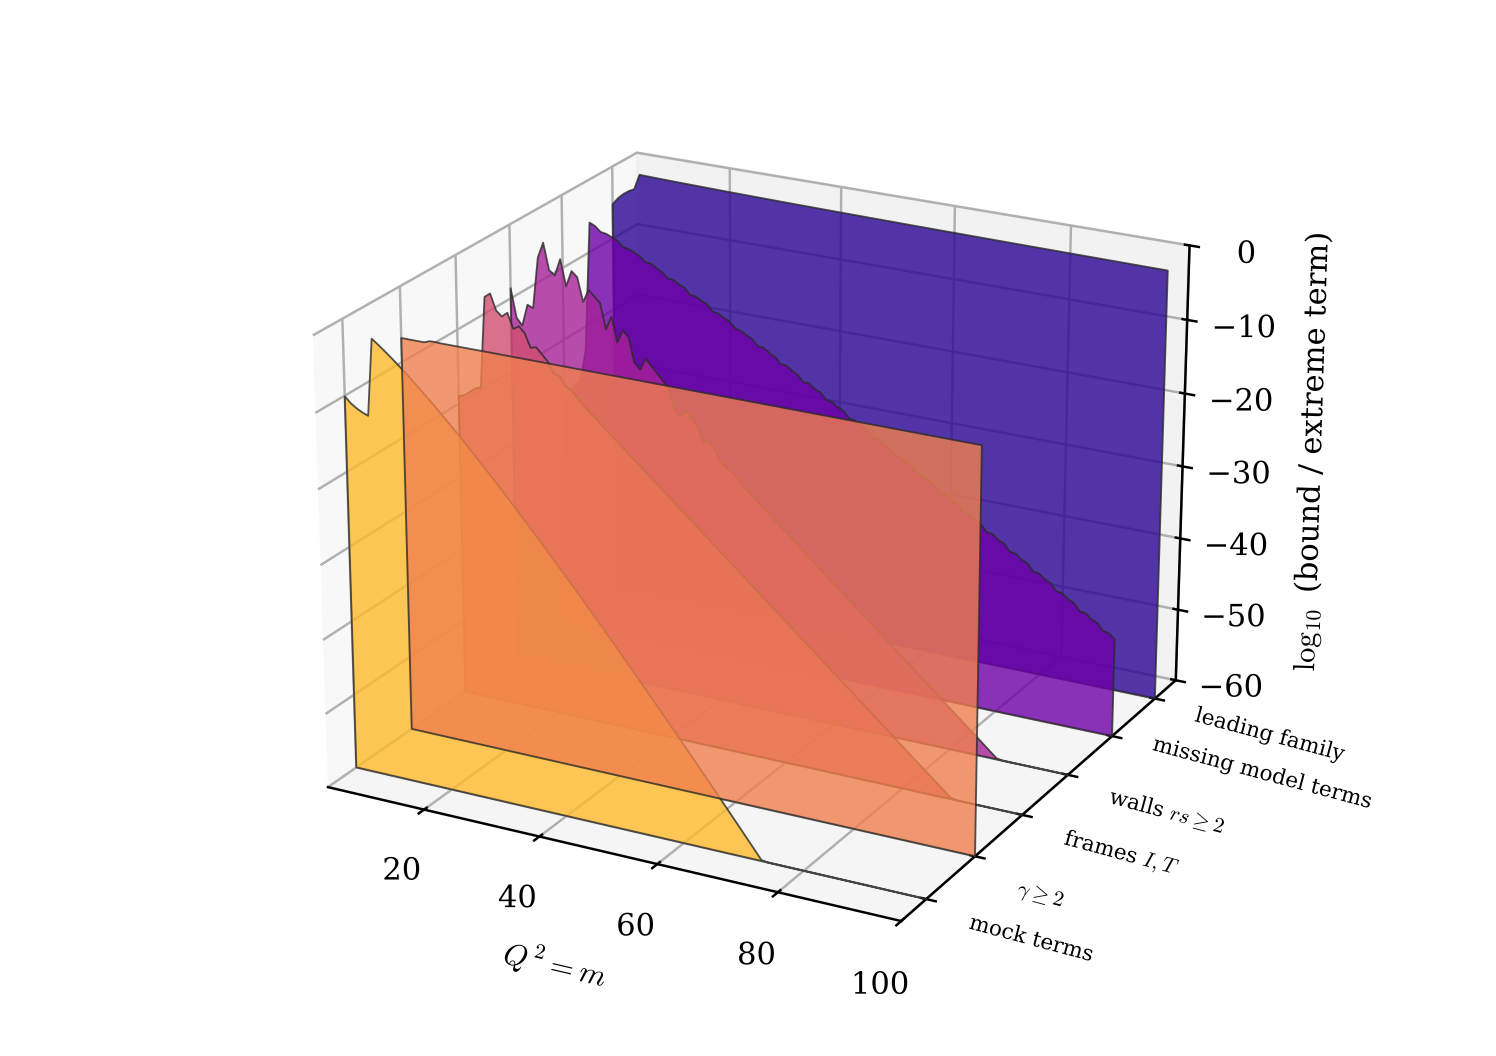
\includegraphics[width=0.84\textwidth]{fig_certificate.png}
\caption{The pieces of the certificate for $3\le Q^2\le100$, on a logarithmic scale and divided by the extreme term $\mathcal E$: shadow terms, terms with $\gamma\ge2$, the frames $I,T$, the walls with $rs\ge2$, the missing model terms and the error of the leading family. Only the last one matters numerically; the others are below $10^{-2}$ at $Q^2=8$ and fall off quickly.}\label{fig:certificate}
\end{figure}

\begin{figure}[t]
\centering
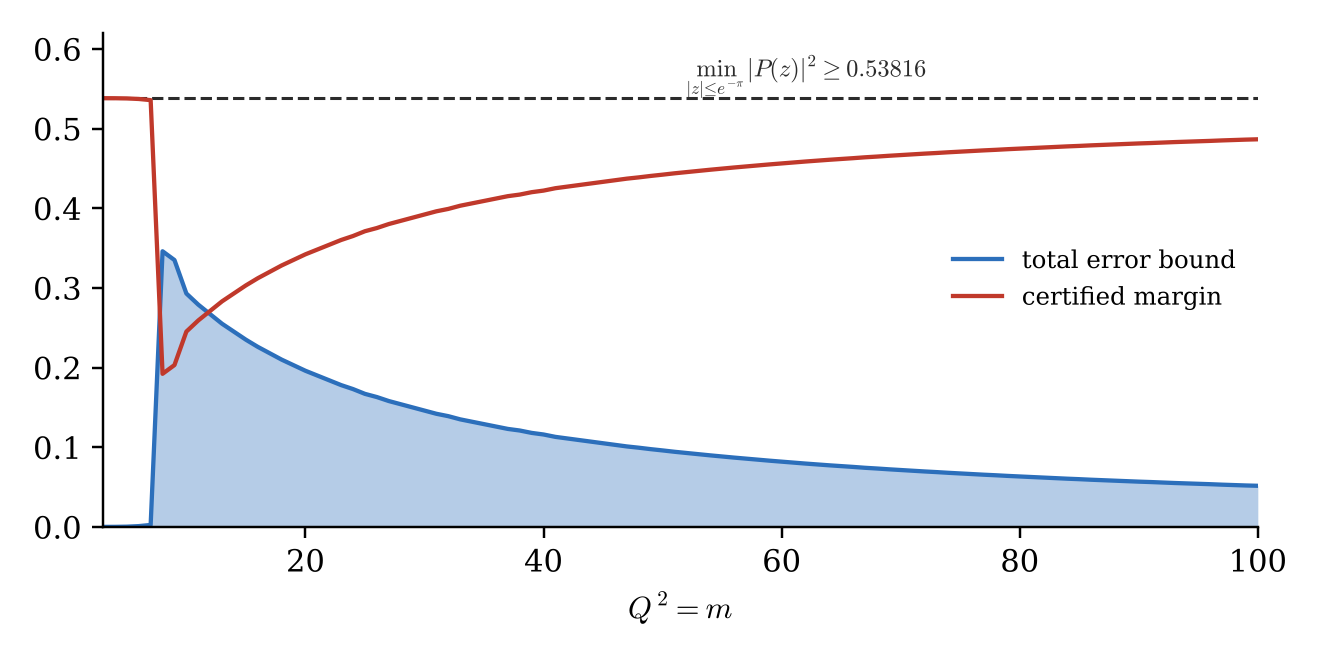
\includegraphics[width=0.8\textwidth]{fig_margins.png}
\caption{The total error bound $\epsilon(m,x_0(m))$ and the margin $0.53816-\epsilon$ for $3\le Q^2\le100$. The margin is smallest at $Q^2=8$, where it is $0.19$.}\label{fig:margins}
\end{figure}

\begin{proof}[Proof of Theorem~\textup{\ref{thm:all}}]
By Proposition~\ref{prop:reduction} it suffices to prove $d^*(m,n,\ell)>0$ for reduced charges. For $m=1,2$ this is Theorem~\ref{thm:main}. Let $m\ge3$. If $m\le7$ and $D\le500$, it is Theorem~\ref{thm:bounded}. Otherwise $x=\sqrt D/m\ge x_0(m)$, with $x_0(m)$ as in Theorem~\ref{thm:cert} for $m\le100$ and $x_0=1$ for $m\ge101$. By \eqref{eq:decomp} and the bounds of Section~\ref{sec:errors}, which are uniform in $x\ge x_0$ and in $\ell$,
\[
\frac{d^*(m,n,\ell)}{\mathcal E(D,m)}\ \ge\ |P(z)|^2-\epsilon(m,x_0)\ \ge\ 0.53816-0.347>0
\]
by Proposition~\ref{prop:pmin} (note $|z|=e^{-\pi x}\le e^{-\pi}$) and Theorems~\ref{thm:cert} and~\ref{thm:analytic}. Since $\mathcal E(D,m)>0$, $d^*(m,n,\ell)>0$.
\end{proof}

\begin{corollary}\label{cor:asym}
Under Hypothesis~\textup{\ref{hyp:R}}, for every reduced charge with $m\ge3$,
\[
0.19\,\mathcal E(D,m)\ \le\ d^*(m,n,\ell)\ \le\ 2.51\,\mathcal E(D,m).
\]
In particular $\log d^*(Q,P)=\pi\sqrt{1+4/Q^2}\,\sqrt{D}-4\log D+O_{Q^2}(1)$ as $D\to\infty$ with $Q^2$ fixed, and $\log d^*=\pi\sqrt{Q^2P^2-(Q\cdot P)^2}+O(\log D)$ when $Q^2\to\infty$ with $\sqrt D/Q^2$ bounded, the Bekenstein--Hawking entropy of the black hole.
\end{corollary}

\begin{proof}
The lower bound is the proof above. For the upper bound, $|P(z)|^2\le P(e^{-\pi})^2\le2.156$ and $\epsilon\le0.347$. The asymptotics follow from \eqref{eq:ext}, $I_\nu(y)\sim e^y/\sqrt{2\pi y}$, and $\pi\sqrt D\,(\sqrt{1+4/m}-1)\le2\pi\sqrt D/m$.
\end{proof}

\begin{remark}\label{rem:sharp}
The minimum $0.5389$ of Proposition~\ref{prop:pmin} is reached in the limit: as $m\to\infty$ along charges with $x=1$ and $\ell=m$ odd, $z=-e^{-\pi}$, and the bounds in the proof of Theorem~\ref{thm:analytic} tend to $0$, since $\varphi(S,m)\to0$ for each fixed $S$. So, under Hypothesis~\ref{hyp:R}, $d^*/\mathcal E$ comes arbitrarily close to $0.5389$, and the factor of the leading family cannot be replaced by a single term; the dominance argument of \cite{Ros24}, with one dominant term, does not carry over to level two without the resummation of Theorem~\ref{thm:model}.
For moderate charges the picture is already accurate: at $Q^2=3$, $P^2/2=10$, $Q\cdot P=3$ the exact index gives $d^*/\mathcal E=0.9485$ while $|P(z)|^2=0.9910$, and at $Q^2=4$, $P^2/2=58$, $Q\cdot P=4$ the two numbers are $0.99990$ and $0.99999$.
\end{remark}


\section{Values and comparison with the product formula}\label{sec:values}

The first single-centred indices given by \eqref{eq:Q1coeff} and \eqref{eq:Q2coeff} are listed in Table~\ref{tab:values}. We expanded the product \eqref{eq:product} in exact rational arithmetic and compared it with \eqref{eq:Q1closed} and \eqref{eq:Q2closed} on every coefficient $x^ey^\ell$ with $e\le 49$ and $|\ell|\le18$; the two sides agree. Every entry of Table~\ref{tab:values} that lies in Sen's Table~2 \cite{Sen11} coincides with it: at $Q^2=1$ the entries $360$, $2164$, $4352$, $18944$, $36024$, $125860$ and the value $2164$ at $(P^2,Q\cdot P)=(6,2)$, and at $Q^2=2$ the entries $198144$, $67008$, $6912$ of the row $P^2=4$ and $1580672$, $671744$, $101376$, $4352$ of the row $P^2=6$.\footnote{In these entries the charge lies in the cone (3.9) of \cite{Sen11}, and the index of the full partition function equals the single-centred index. The entries of Sen's table with $D\le0$, such as $-2$ at $(Q^2,P^2,Q\cdot P)=(1,2,2)$ or $-16$ at $(2,6,4)$, are outside the scope of the theorem, as they should be.} Figure~\ref{fig:indices} shows $\log_{10}d^*$ on the two rows.

\begin{table}[t]
\centering
\small
\begin{tabular}{@{}cr@{\qquad}cr@{\qquad}cr@{\qquad}cr@{}}
\toprule
\multicolumn{2}{c}{$Q^2=1$} & \multicolumn{6}{c}{$Q^2=2$}\\
\cmidrule(r){1-2}\cmidrule(l){3-8}
$D$ & $d^*$ & $D$ & $d^*$\ ($\ell$ odd) & $D$ & $d^*$\ ($\ell\equiv0$) & $D$ & $d^*$\ ($\ell\equiv2$)\\
\midrule
1 & 360 & 3 & 4352 & 4 & 18944 & 4 & 6912\\
2 & 2164 & 7 & 67008 & 8 & 198144 & 8 & 101376\\
3 & 4352 & 11 & 671744 & 12 & 1580672 & 12 & 992256\\
4 & 18944 & 15 & 5189696 & 16 & 10586880 & 16 & 7550400\\
5 & 36024 & 19 & 33581312 & 20 & 62035968 & 20 & 48253952\\
6 & 125860 & 23 & 190095232 & 24 & 327011328 & 24 & 270195712\\
7 & 233080 & 27 & 968248576 & 28 & 1578794128 & 28 & 1362534400\\
8 & 705536 & 31 & 4522209472 & 32 & 7075522048 & 32 & 6304638848\\
\bottomrule
\end{tabular}
\caption{The first single-centred indices on the rows $Q^2=1$ and $Q^2=2$, as functions of $D=Q^2P^2-(Q\cdot P)^2$ and, at $Q^2=2$, of $\ell=Q\cdot P$ modulo $4$.}\label{tab:values}
\end{table}

\begin{figure}[t]
\centering
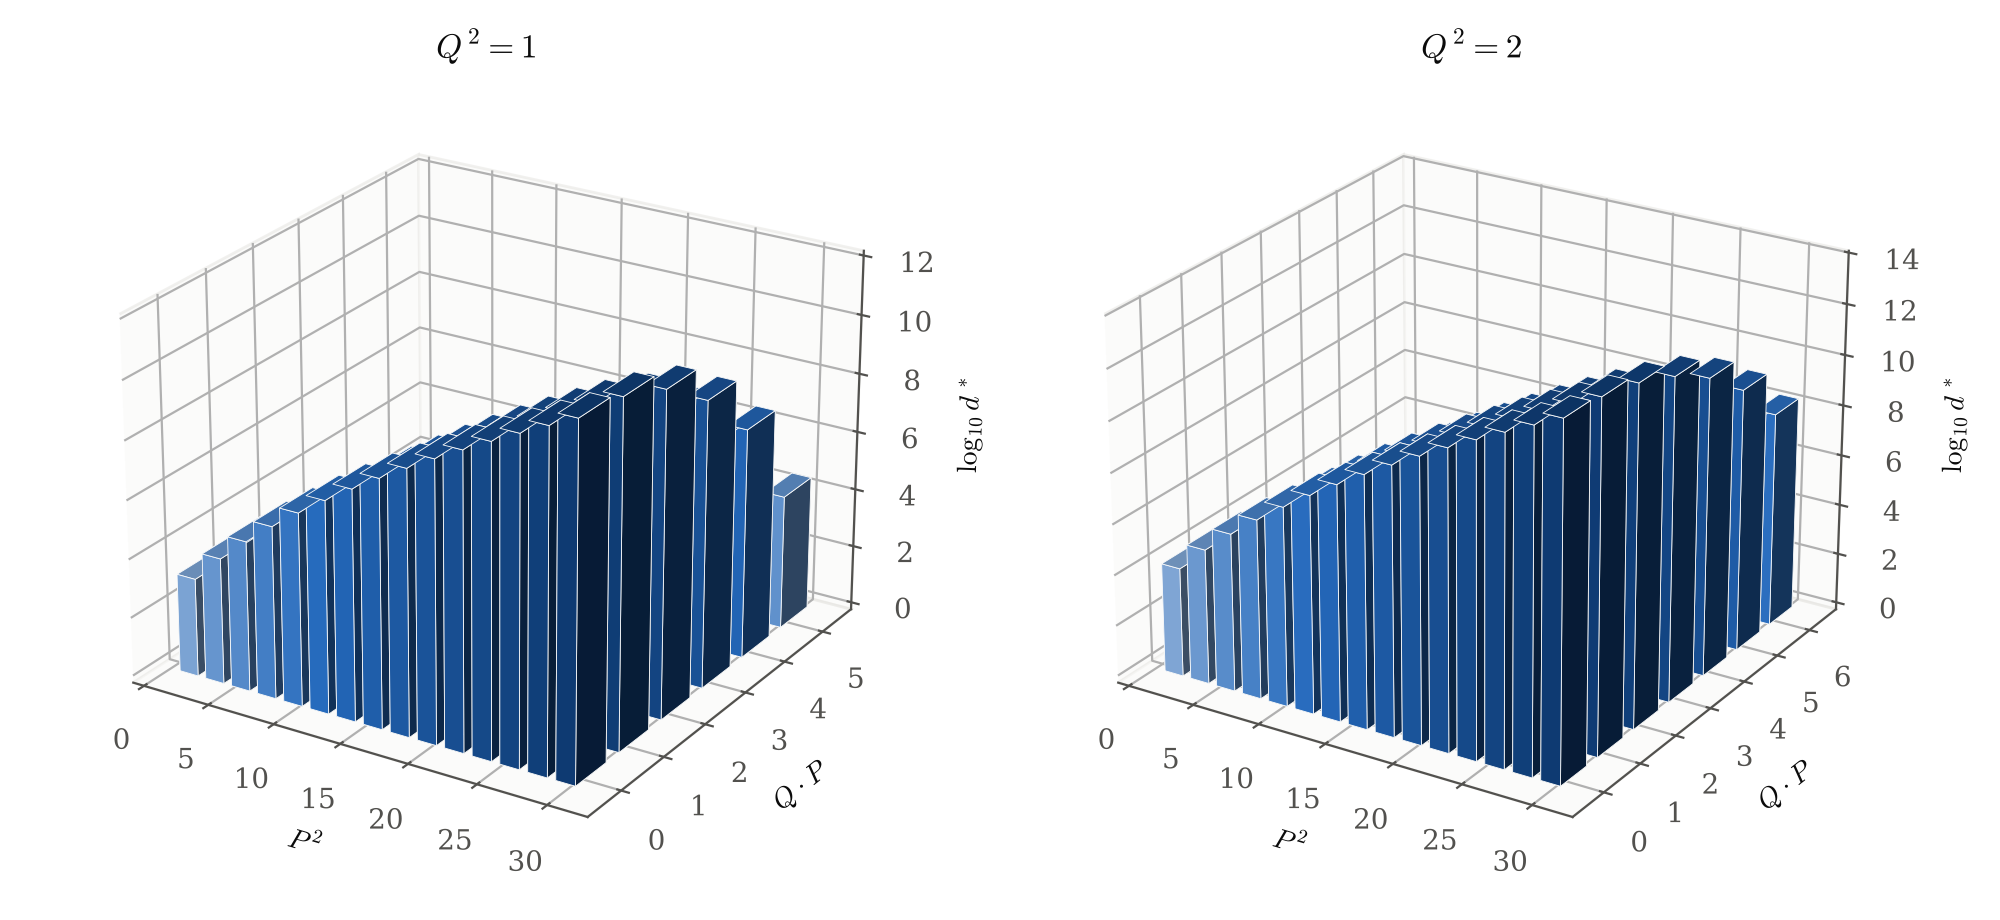
\includegraphics[width=\textwidth]{fig_indices.png}
\caption{$\log_{10}d^*(Q,P)$ for $Q^2=1$ (left) and $Q^2=2$ (right), $2\le P^2\le30$ and $0\le Q\cdot P\le\min(6,P^2)$ with $Q^2P^2>(Q\cdot P)^2$. Every bar is positive, as Theorems~\ref{thm:Q1} and~\ref{thm:Q2} assert.}\label{fig:indices}
\end{figure}

\begin{remark}\label{rem:Q3}
At $Q^2=3$, where $\hat f(3)=1122$, positivity holds for $D\le\Dexact$ by Theorem~\ref{thm:bounded} and for all $D$ under Hypothesis~\ref{hyp:R} by Theorem~\ref{thm:all}. An unconditional proof along the lines of Sections~\ref{sec:Q1} and~\ref{sec:Q2} would need the closed form of $\varphi_3$. The coefficients of the product formula that we computed (all $x^ey^\ell$ with $e<60$) are matched by $g(\frac\sigma2)\varphi_3=1122\,\varphi^{\rm opt}_{2,3}+J_3=1122\,\mathcal A_{2,3}-1122\,\cH|V_3+J_3$, with $\varphi^{\rm opt}_{2,3}$ the form of \cite[(9.12)--(9.13)]{DMZ12} and $J_3$ a holomorphic Jacobi form of weight two and index three built from $A$, $B$ and Eisenstein series at $\sigma$ and $\sigma/2$. Proving this identity needs the analogue of Proposition~\ref{prop:P3} at index four, and the signs of the theta components of $J_3$ would then have to be determined.
\end{remark}

\section{What remains}\label{sec:remains}

The proof of Theorem~\ref{thm:all} uses Hypothesis~\ref{hyp:R} and nothing else that is unproved. Three routes would remove it.
\begin{enumerate}
\item[(1)] \emph{The expansion (H).} The method of Bringmann and Manschot \cite{BMa13} writes a mixed mock Jacobi form as a combination of Poincar\'e series and of the image of the shadow under a non-holomorphic Eichler integral, and proves that the difference is a cusp form of positive weight that vanishes for weight reasons. At level two the Poincar\'e series have to be summed over the three frames, and the vanishing argument has to be made for $\Gamma^0(2)$; the space of holomorphic cusp forms that could intervene has weight $6+\frac12$ in each theta component, and its vanishing is the one point that needs an idea. The agreement to $21$ digits at $Q^2=1,2$ (Section~\ref{ssec:evidence}) shows that no such cusp form is present there.
\item[(2)] \emph{The polar data (P0), (P$\infty$).} Cardoso, Nampuri and Rossell\'o derive the continued-fraction formula \cite[(2.43)]{CNR21} by tracking the poles of $1/\Phit_k$ across the walls of marginal stability. The same contour argument, applied to $\varphi^F_m$ transformed by $\sigma\mapsto-1/\sigma$, would give (P0); (P$\infty$) is its restriction to the walls fixed by the half shift.
\item[(3)] \emph{Exact computation.} Each further unit of $Q^2$ for which the remainder $J_m$ has a closed form, as at $Q^2=1,2$, removes the hypothesis on that row. Theorem~\ref{thm:cert} shows that the margin for $3\le Q^2\le7$ is above $0.53$ as soon as $D>500$, so on these rows the analytic picture of Section~\ref{sec:model} is already in force at moderate discriminant.
\end{enumerate}
The method itself is not special to $N=2$. For the $\ZZ_N$ CHL models with $N=3,5,7$ the leading family of walls again resums, now to $|1/\eta(\tau)^{k+2}\eta(N\tau)^{k+2}|^2$ evaluated at $e^{-2\pi x/N+i\theta}$ with $k+2=24/(N+1)$, and positivity reduces in the same way to a lower bound for this modulus and to an expansion of type (H) at level $N$.


\section*{Declarations}

\subsection*{Data availability}
The programs and data that support the findings of this study are openly available in the archive \cite{Bha26c}, at \url{https://doi.org/\zenodoDOI}. They comprise the exact computation of Appendix~\ref{app:exact}, the interval certificates of Appendix~\ref{app:interval}, the checks of Section~\ref{ssec:evidence}, the programs that verify Propositions~\ref{prop:Q1closed}, \ref{prop:P3} and~\ref{prop:Q2closed} and the values of Table~\ref{tab:values}, and the scripts that draw the figures.

\subsection*{Funding}
No funding was received for conducting this study.

\subsection*{Conflict of interest}
The author has no conflicts of interest to declare that are relevant to the content of this article.

\subsection*{Ethics statement}
This study involves no human participants, animals or personal data; no ethical approval was required.


\appendix

\section{The exact computation}\label{app:exact}

The program \texttt{chl\_coefficients.py} of the archive \cite{Bha26c} proves Theorem~\ref{thm:bounded} in exact integer arithmetic, in five steps.
\begin{enumerate}
\item[(B1)] \emph{Orbits.} A charge $(m,n,\ell)$ corresponds to the binary quadratic form $f(s,t)=ms^2+2\ell st+2nt^2$ of discriminant $-8D$, and $\Gamma_1(2)$ acts by $f\mapsto f\circ g$. The orbits with given $D$ are enumerated through the Gauss-reduced forms of discriminant $-8D$, each with a class of bottom rows modulo $2$, taken modulo the automorphs of the reduced form.
\item[(B2)] \emph{A representative in $\mathcal A$.} In every orbit the program finds a charge with $0\le\ell<2m$ satisfying \eqref{eq:setA}, which it tests in the form $2(jm+\ell m_1)^2+m_1^2\cdot2D\ge2m^2$ for $m_1\in2\ZZ\setminus\{0\}$ and odd $j$ with $m_1\mid(j^2-1)/4$, the range of $(m_1,j)$ being finite because the left side grows.
\item[(B3)] \emph{Coefficients.} The coefficients $c_{\mathcal R}(m,n,\ell)$ are computed from \eqref{eq:product} by the recursion for the exponential of \eqref{eq:Ll}, with polynomial products in FLINT \cite{Har10}. By Lemma~\ref{lem:chamber}(ii) each charge is read in the cheaper of its two orientations.
\item[(B4)] \emph{Signs.} For every orbit, $d^*=(-1)^{\ell+1}c_{\mathcal R}(m,n,\ell)$ is computed for every representative found in the box, the values are compared, and the sign is checked. At $m=1,2$ the values are compared with Propositions~\ref{prop:Q1closed} and~\ref{prop:Q2closed}.
\item[(B5)] \emph{Least representatives.} On the whole range, every charge of least $Q^2$ in its orbit is checked to lie in $\mathcal A$, as Lemma~\ref{lem:leastA} predicts.
\end{enumerate}
For $D\le\Dexact$ there are $\Norbits$ orbits, with $Q^2\le\Qmaxexact$ for the least representative; all have $d^*>0$. The smallest value relative to the extreme term occurs at small $D$, where $x$ is close to $1$; this is the region in which the leading-family error of Lemma~\ref{lem:mainerr} is largest and which Theorem~\ref{thm:bounded} covers for $Q^2\le7$.

\section{Interval computations}\label{app:interval}

All the numerical statements used in the proofs are certified in ball arithmetic with Arb \cite{Joh17} through python-flint; each program prints its enclosures.
\begin{enumerate}
\item[(I1)] \texttt{pmin.py}: Proposition~\ref{prop:pmin}. Product truncated at $n=60$ with an explicit tail enclosure, $4001$ points on the half circle, Lipschitz constant $L=2P(r_0)r_0P'(r_0)$.
\item[(I2)] \texttt{gmono2.py}: Lemma~\ref{lem:gfacts}. Monotonicity of $\phi$ on $[3,60]$ by mean-value enclosures on an adaptive cover; the range $[60,\infty)$ through the closed form \eqref{eq:halfint}.
\item[(I3)] \texttt{cert.py}: Theorem~\ref{thm:cert}. For each $m$ the program lists the leading family $\mathcal L_m$, the walls with $rs\ge2$ and the parity walls through their parameters $(r,s,a,b)$, encloses $t(r,s,a,b)$, and evaluates the seven bounds of Section~\ref{sec:errors}. In \eqref{eq:XT} it uses $32$ in place of $16$.
\item[(I4)] \texttt{analytic.py}, \texttt{analytic2.py}: Theorem~\ref{thm:analytic}.
\item[(I5)] \texttt{polar.py}: the wall sums \eqref{eq:P0}, \eqref{eq:Pinf}, used also for the checks (c), (d) of Section~\ref{ssec:evidence}.
\end{enumerate}

\section{The certified margins}\label{app:margins}

Table~\ref{tab:margins} lists, for $3\le Q^2\le100$, the total bound $\epsilon(m,x_0(m))$ of Theorem~\ref{thm:cert} and the margin $0.53816-\epsilon$.

\begin{table}[ht]
\centering
\footnotesize
\setlength{\tabcolsep}{3.5pt}
\caption{The certified total error $\epsilon(m,x_0(m))$ of Theorem~\ref{thm:cert} and the margin $0.53816-\epsilon$, for $m=Q^2$.}\label{tab:margins}
\begin{tabular}{rll|rll|rll|rll}
\hline
$m$ & $\epsilon$ & margin & $m$ & $\epsilon$ & margin & $m$ & $\epsilon$ & margin & $m$ & $\epsilon$ & margin \\
\hline
3 & $6.04\cdot10^{-6}$ & 0.5380 & 28 & 0.1540 & 0.3842 & 53 & 0.0913 & 0.4467 & 78 & 0.0648 & 0.4732 \\
4 & $5.47\cdot10^{-5}$ & 0.5379 & 29 & 0.1500 & 0.3883 & 54 & 0.0898 & 0.4482 & 79 & 0.0640 & 0.4740 \\
5 & $2.87\cdot10^{-4}$ & 0.5377 & 30 & 0.1460 & 0.3921 & 55 & 0.0884 & 0.4496 & 80 & 0.0633 & 0.4747 \\
6 & $9.79\cdot10^{-4}$ & 0.5370 & 31 & 0.1420 & 0.3958 & 56 & 0.0870 & 0.4510 & 81 & 0.0626 & 0.4754 \\
7 & 0.0024 & 0.5356 & 32 & 0.1390 & 0.3993 & 57 & 0.0857 & 0.4523 & 82 & 0.0619 & 0.4761 \\
8 & 0.3460 & 0.1917 & 33 & 0.1350 & 0.4026 & 58 & 0.0844 & 0.4536 & 83 & 0.0612 & 0.4768 \\
9 & 0.3350 & 0.2030 & 34 & 0.1320 & 0.4058 & 59 & 0.0831 & 0.4549 & 84 & 0.0605 & 0.4775 \\
10 & 0.2930 & 0.2450 & 35 & 0.1290 & 0.4089 & 60 & 0.0819 & 0.4561 & 85 & 0.0599 & 0.4781 \\
11 & 0.2790 & 0.2594 & 36 & 0.1260 & 0.4118 & 61 & 0.0807 & 0.4573 & 86 & 0.0592 & 0.4788 \\
12 & 0.2670 & 0.2714 & 37 & 0.1230 & 0.4145 & 62 & 0.0795 & 0.4585 & 87 & 0.0586 & 0.4794 \\
13 & 0.2550 & 0.2828 & 38 & 0.1210 & 0.4172 & 63 & 0.0784 & 0.4596 & 88 & 0.0580 & 0.4800 \\
14 & 0.2450 & 0.2930 & 39 & 0.1180 & 0.4197 & 64 & 0.0773 & 0.4607 & 89 & 0.0574 & 0.4806 \\
15 & 0.2350 & 0.3026 & 40 & 0.1160 & 0.4222 & 65 & 0.0763 & 0.4617 & 90 & 0.0568 & 0.4812 \\
16 & 0.2260 & 0.3115 & 41 & 0.1130 & 0.4245 & 66 & 0.0753 & 0.4627 & 91 & 0.0563 & 0.4817 \\
17 & 0.2180 & 0.3199 & 42 & 0.1110 & 0.4268 & 67 & 0.0742 & 0.4638 & 92 & 0.0557 & 0.4823 \\
18 & 0.2100 & 0.3277 & 43 & 0.1090 & 0.4289 & 68 & 0.0733 & 0.4647 & 93 & 0.0551 & 0.4829 \\
19 & 0.2030 & 0.3350 & 44 & 0.1070 & 0.4310 & 69 & 0.0723 & 0.4657 & 94 & 0.0546 & 0.4834 \\
20 & 0.1960 & 0.3419 & 45 & 0.1050 & 0.4330 & 70 & 0.0714 & 0.4666 & 95 & 0.0541 & 0.4839 \\
21 & 0.1900 & 0.3483 & 46 & 0.1030 & 0.4350 & 71 & 0.0705 & 0.4675 & 96 & 0.0536 & 0.4844 \\
22 & 0.1840 & 0.3544 & 47 & 0.1010 & 0.4368 & 72 & 0.0696 & 0.4684 & 97 & 0.0530 & 0.4850 \\
23 & 0.1780 & 0.3601 & 48 & 0.0994 & 0.4386 & 73 & 0.0688 & 0.4692 & 98 & 0.0525 & 0.4855 \\
24 & 0.1730 & 0.3655 & 49 & 0.0976 & 0.4404 & 74 & 0.0679 & 0.4701 & 99 & 0.0520 & 0.4860 \\
25 & 0.1670 & 0.3706 & 50 & 0.0960 & 0.4420 & 75 & 0.0671 & 0.4709 & 100 & 0.0516 & 0.4864 \\
26 & 0.1630 & 0.3754 & 51 & 0.0943 & 0.4437 & 76 & 0.0663 & 0.4717 &  & &  \\
27 & 0.1580 & 0.3799 & 52 & 0.0928 & 0.4452 & 77 & 0.0655 & 0.4725 &  & &  \\
\hline
\end{tabular}
\end{table}



\begin{thebibliography}{99}

\bibitem{BEW98} B.~C.~Berndt, R.~J.~Evans, K.~S.~Williams, \emph{Gauss and Jacobi Sums}, Canadian Mathematical Society Series of Monographs and Advanced Texts, Wiley, New York, 1998.

\bibitem{Bha22} D.~Bhattacharjee, \emph{Generalization of quartic and quintic Calabi--Yau manifolds fibered by polarized K3 surfaces}, Research Square (2022). doi:10.21203/rs.3.rs-1965255/v1

\bibitem{Bha26c} D.~Bhattacharjee, \emph{Code and data for: Positivity of single-centred black hole indices in the $\mathbb Z_2$ CHL model}, Zenodo (2026). doi:\zenodoDOI

\bibitem{BM13} K.~Bringmann, S.~Murthy, \emph{On the positivity of black hole degeneracies in string theory}, Commun. Number Theory Phys. \textbf{7} (2013), 15--56. doi:10.4310/CNTP.2013.v7.n1.a2

\bibitem{BMa13} K.~Bringmann, J.~Manschot, \emph{From sheaves on $\mathbb P^2$ to a generalization of the Rademacher expansion}, Amer. J. Math. \textbf{135} (2013), 1039--1065. doi:10.1353/ajm.2013.0031

\bibitem{BN26} D.~Bhattacharjee, P.~Nandi, \emph{Enriques and Kummer surfaces arising from K3 involutions}, Preprints (2026). doi:10.20944/preprints202602.0098.v1

\bibitem{BSS25} A.~Bhand, A.~Sen, R.~K.~Singh, \emph{Mock modularity in CHL models}, Res. Math. Sci. \textbf{12} (2025), 8. doi:10.1007/s40687-024-00489-0

\bibitem{CHL95} S.~Chaudhuri, G.~Hockney, J.~D.~Lykken, \emph{Maximally supersymmetric string theories in $D<10$}, Phys. Rev. Lett. \textbf{75} (1995), 2264--2267. doi:10.1103/PhysRevLett.75.2264

\bibitem{CNR21} G.~L.~Cardoso, S.~Nampuri, M.~Rossell\'o, \emph{Arithmetic of decay walls through continued fractions: a new exact dyon counting solution in $\mathcal N=4$ CHL models}, J. High Energy Phys. \textbf{2021}, no.~3 (2021), 154. doi:10.1007/JHEP03(2021)154

\bibitem{Coc67} J.~A.~Cochran, \emph{The monotonicity of modified Bessel functions with respect to their order}, J. Math. and Phys. \textbf{46} (1967), 220--222.

\bibitem{CV08} M.~C.~N.~Cheng, E.~P.~Verlinde, \emph{Wall crossing, discrete attractor flow and Borcherds algebra}, SIGMA \textbf{4} (2008), 068. doi:10.3842/SIGMA.2008.068

\bibitem{DJS06} J.~R.~David, D.~P.~Jatkar, A.~Sen, \emph{Product representation of dyon partition function in CHL models}, J. High Energy Phys. \textbf{2006}, no.~6 (2006), 064. doi:10.1088/1126-6708/2006/06/064

\bibitem{DMZ12} A.~Dabholkar, S.~Murthy, D.~Zagier, \emph{Quantum black holes, wall crossing and mock modular forms}, arXiv:1208.4074 (2012).

\bibitem{DN07} A.~Dabholkar, S.~Nampuri, \emph{Spectrum of dyons and black holes in CHL orbifolds using Borcherds lift}, J. High Energy Phys. \textbf{2007}, no.~11 (2007), 077. doi:10.1088/1126-6708/2007/11/077

\bibitem{DS06} J.~R.~David, A.~Sen, \emph{CHL dyons and statistical entropy function from D1-D5 system}, J. High Energy Phys. \textbf{2006}, no.~11 (2006), 072. doi:10.1088/1126-6708/2006/11/072

\bibitem{DVV97} R.~Dijkgraaf, E.~Verlinde, H.~Verlinde, \emph{Counting dyons in $N=4$ string theory}, Nucl. Phys. B \textbf{484} (1997), 543--561. doi:10.1016/S0550-3213(96)00640-2

\bibitem{EZ85} M.~Eichler, D.~Zagier, \emph{The Theory of Jacobi Forms}, Progress in Mathematics \textbf{55}, Birkh\"auser, Boston, 1985. doi:10.1007/978-1-4684-9162-3

\bibitem{FR17} G.~Ferrari, V.~Reys, \emph{Mixed Rademacher and BPS black holes}, J. High Energy Phys. \textbf{2017}, no.~7 (2017), 094. doi:10.1007/JHEP07(2017)094

\bibitem{GN97} V.~A.~Gritsenko, V.~V.~Nikulin, \emph{Siegel automorphic form corrections of some Lorentzian Kac--Moody Lie algebras}, Amer. J. Math. \textbf{119} (1997), 181--224. arXiv:alg-geom/9504006

\bibitem{Har10} W.~B.~Hart, \emph{Fast Library for Number Theory: an introduction}, in: Mathematical Software -- ICMS 2010, Lecture Notes in Comput. Sci. \textbf{6327}, Springer, Berlin, 2010, 88--91. doi:10.1007/978-3-642-15582-6\_18

\bibitem{Joh17} F.~Johansson, \emph{Arb: efficient arbitrary-precision midpoint-radius interval arithmetic}, IEEE Trans. Comput. \textbf{66} (2017), 1281--1292. doi:10.1109/TC.2017.2690633

\bibitem{JS06} D.~P.~Jatkar, A.~Sen, \emph{Dyon spectrum in CHL models}, J. High Energy Phys. \textbf{2006}, no.~4 (2006), 018. doi:10.1088/1126-6708/2006/04/018

\bibitem{PV15} D.~Persson, R.~Volpato, \emph{Fricke S-duality in CHL models}, J. High Energy Phys. \textbf{2015}, no.~12 (2015), 156. doi:10.1007/JHEP12(2015)156

\bibitem{Ros24} M.~Rossell\'o, \emph{The immortal dyon index is positive}, arXiv:2403.19630 (2024).

\bibitem{RZ38} H.~Rademacher, H.~S.~Zuckerman, \emph{On the Fourier coefficients of certain modular forms of positive dimension}, Ann. of Math. \textbf{39} (1938), 433--462. doi:10.2307/1968796

\bibitem{SBBT26} R.~Sadhu, D.~Bhattacharjee, S.~Bhattacharya, S.~N.~Thakur, \emph{$E_8\times E_8$ heterotic gravity and M-theory}, SSRN (2026). doi:10.2139/ssrn.6326718

\bibitem{Sen07} A.~Sen, \emph{Walls of marginal stability and dyon spectrum in $\mathcal N=4$ supersymmetric string theories}, J. High Energy Phys. \textbf{2007}, no.~5 (2007), 039. doi:10.1088/1126-6708/2007/05/039

\bibitem{Sen08} A.~Sen, \emph{Black hole entropy function, attractors and precision counting of microstates}, Gen. Relativ. Gravit. \textbf{40} (2008), 2249--2431. doi:10.1007/s10714-008-0626-4

\bibitem{Sen11} A.~Sen, \emph{How do black holes predict the sign of the Fourier coefficients of Siegel modular forms?}, Gen. Relativ. Gravit. \textbf{43} (2011), 2171--2183. doi:10.1007/s10714-011-1175-9

\bibitem{Sin26} R.~K.~Singh, \emph{Generating function of single-centered black hole index in CHL models}, arXiv:2606.19479 (2026).

\bibitem{SSY06} D.~Shih, A.~Strominger, X.~Yin, \emph{Recounting dyons in $\mathcal N=4$ string theory}, J. High Energy Phys. \textbf{2006}, no.~10 (2006), 087. doi:10.1088/1126-6708/2006/10/087

\bibitem{Stu87} J.~Sturm, \emph{On the congruence of modular forms}, in: Number Theory (New York, 1984--85), Lecture Notes in Math. \textbf{1240}, Springer, Berlin, 1987, 275--280. doi:10.1007/BFb0072985

\bibitem{Wat44} G.~N.~Watson, \emph{A Treatise on the Theory of Bessel Functions}, 2nd ed., Cambridge University Press, Cambridge, 1944.

\bibitem{WW21} E.~T.~Whittaker, G.~N.~Watson, \emph{A Course of Modern Analysis}, 5th ed., Cambridge University Press, Cambridge, 2021. doi:10.1017/9781009004091

\bibitem{Zag08} D.~Zagier, \emph{Elliptic modular forms and their applications}, in: The 1-2-3 of Modular Forms, Universitext, Springer, Berlin, 2008, 1--103. doi:10.1007/978-3-540-74119-0\_1

\bibitem{Zuc39} H.~S.~Zuckerman, \emph{On the coefficients of certain modular forms belonging to subgroups of the modular group}, Trans. Amer. Math. Soc. \textbf{45} (1939), 298--321. doi:10.1090/S0002-9947-1939-1501993-X

\bibitem{Zwe02} S.~Zwegers, \emph{Mock Theta Functions}, PhD thesis, Universiteit Utrecht, 2002. arXiv:0807.4834

\end{thebibliography}

\end{document}
